\documentclass[11pt]{article}
\usepackage[T1]{fontenc}
\usepackage{lmodern}
\usepackage[margin=1in]{geometry}
\usepackage{amsmath,amssymb,amsthm,mathtools}
\usepackage{microtype,enumitem,booktabs,longtable,array}
\usepackage{xcolor,tikz}
\usetikzlibrary{arrows.meta,positioning,automata,calc}
\usepackage[numbers,sort&compress]{natbib}
\usepackage[colorlinks=true,linkcolor=blue!50!black,citecolor=blue!50!black,urlcolor=blue!50!black]{hyperref}
\hypersetup{pdftitle={Arithmetic classification and non-Pisot singularity for Bernoulli convolutions},pdfauthor={OpenAI}}
\newtheorem{theorem}{Theorem}[section]
\newtheorem{lemma}[theorem]{Lemma}
\newtheorem{proposition}[theorem]{Proposition}
\newtheorem{corollary}[theorem]{Corollary}
\theoremstyle{definition}
\newtheorem{definition}[theorem]{Definition}
\theoremstyle{remark}
\newtheorem{remark}[theorem]{Remark}
\newcommand{\R}{\mathbb R}
\newcommand{\C}{\mathbb C}
\newcommand{\Z}{\mathbb Z}
\newcommand{\N}{\mathbb N}
\newcommand{\Q}{\mathbb Q}
\newcommand{\E}{\mathbb E}
\newcommand{\Pbb}{\mathbb P}
\DeclareMathOperator{\dist}{dist}
\DeclareMathOperator{\supp}{supp}
\DeclareMathOperator{\Var}{Var}
\numberwithin{equation}{section}
\title{Arithmetic classification and non-Pisot singularity\newline for Bernoulli convolutions}
\author{OpenAI}
\date{October 3, 2026}
\begin{document}
\maketitle
\begin{abstract}
We give an arithmetic classification of singular and absolutely continuous unbiased Bernoulli convolutions for every parameter $\lambda\in(0,1)$. The criterion is expressed through one-sided approximation by explicitly defined finite sets of algebraic units; it is an infinite approximation condition, not a finite membership algorithm. We also establish singular examples beyond reciprocals of Pisot numbers: singularity holds at the reciprocal of every quartic Salem number in $(1,2)$ and at the reciprocal of a specified non-Pisot root of an explicit degree-$31$ polynomial.
\end{abstract}

\section{Introduction}\label{sec:introduction}
For $0<\lambda<1$, the unbiased Bernoulli convolution $\nu_\lambda$ is the law of
\begin{equation}\label{intro:series}
 Y_\lambda=\sum_{n=0}^{\infty}\varepsilon_n\lambda^n,
 \qquad \Pbb(\varepsilon_n=1)=\Pbb(\varepsilon_n=-1)=\tfrac12,
\end{equation}
where the signs are independent. The series converges absolutely. We also use the bit form $\mu_\lambda$, the law of
\[
 X_\lambda=\sum_{n=0}^{\infty}u_n\lambda^n,
 \qquad \Pbb(u_n=0)=\Pbb(u_n=1)=\tfrac12.
\]
The relation $Y_\lambda=2X_\lambda-(1-\lambda)^{-1}$ preserves singularity and absolute continuity. A measure is singular if it gives full mass to a Borel set of Lebesgue measure zero. Bernoulli convolutions have pure type: they are either singular or absolutely continuous \cite[Theorem~11]{JessenWintner1935}. The classification problem asks which of these alternatives holds for each parameter, including exceptional parameters.

For $\lambda<1/2$, a direct interval cover proves singularity; at $\lambda=1/2$, $\nu_\lambda$ is uniform on $[-2,2]$. The interval $(1/2,1)$ presents the arithmetic difficulty. A \emph{Pisot number} is a real algebraic integer $\beta>1$ whose other conjugates have modulus less than one. Erd\H{o}s proved singularity when $\lambda^{-1}$ is Pisot by showing that the Fourier transform does not tend to zero \cite{Erdos1939}. Garsia subsequently established absolute continuity for a different arithmetic class, including reciprocals of algebraic integers of absolute norm two whose conjugates all have modulus greater than one \cite{Garsia1962}.

The almost-everywhere theory gives a complementary picture. Solomyak proved that $\nu_\lambda$ has an $L^2$ density for Lebesgue-almost every $\lambda\in(1/2,1)$ \cite{Solomyak1995}. Hochman's work relates dimension loss to very strong concentration of cylinder positions \cite{Hochman2014}, and Shmerkin proved that the possible singular parameters in this interval form a set of Hausdorff dimension zero \cite{Shmerkin2014}. Varj\'u proved full dimension for every transcendental parameter in this interval \cite{VarjuTranscendental2019}. These conclusions leave measure type at exceptional parameters to be resolved; full dimension alone does not imply absolute continuity. The survey \cite{PeresSchlagSolomyak2000} describes the classical development and the roles of arithmetic, overlap, and Fourier decay.

Garsia connected singularity with entropy of finite sums \cite{Garsia1963}. Algebraic approximation also plays a central role in the dimension theory: Breuillard and Varj\'u showed that a dimension-deficient parameter can be approximated exceptionally closely by algebraic parameters whose Bernoulli convolutions also have dimension less than one \cite[Theorem~1]{BreuillardVarju2019}. The criterion below addresses measure type and also records the number and coefficient directions of nearby algebraic targets.

A \emph{Salem number} is a real algebraic integer $\beta>1$ whose other conjugates consist of $\beta^{-1}$ and conjugates on the unit circle. In degree four there is a single nonreal conjugate pair. Salem proved that the Fourier transform of $\nu_\lambda$ tends to zero whenever $\lambda^{-1}$ is not Pisot \cite{Salem1943}. Thus Fourier nondecay cannot prove singularity for Salem parameters. Marshall-Maldonado and Solomyak recently obtained quantitative decay estimates for these convolutions \cite[Appendix~B]{MarshallMaldonadoSolomyak2026}; those estimates do not decide absolute continuity. The existence of singular examples with non-Pisot reciprocal is explicitly recorded as open in the recent literature \cite{BakerEtAl2026,KernSterk2026}.

This paper gives an arithmetic criterion for every parameter and proves two classes of non-Pisot singularity results. The criterion in Theorem~\ref{cls:classification} uses finite sets of real algebraic units. Their minimal polynomials have coefficients in $\{-1,0,1\}$, prescribed degree, and irreducible reduction modulo two. A target unit is retained when nearby units supply sufficiently many distinct initial coefficient vectors in a fixed positive proportion of the coordinate orthants. Singularity is equivalent to one-sided approximation by these retained targets at a fixed geometric rate. All target sets are defined by finite polynomial algebra; their construction uses no information about the type of any Bernoulli convolution. The resulting classification is an approximation property, and need not provide a short test for membership at a given real parameter.

The main step behind the criterion is a realization lemma. Concentration of the measure produces many pairs of finite bit words with nearby sums and different first bits. Their difference vectors can be completed to height-one polynomials having a root strictly above the parameter. A uniform finite-order nonvanishing estimate preserves a sign change, while prime polynomials in arithmetic progressions over $\mathbb F_2$ supply irreducibility without altering the initial coefficients. This separates the concentration argument from the algebraic realization, and gives a way to translate overlap information into constrained algebraic approximation.

The two non-Pisot results are proved directly; the criterion then yields the corresponding approximation properties. Theorem~\ref{sal:main} proves singularity for the reciprocal of every quartic Salem number in $(1,2)$. We construct algebraic multipliers whose unit-circle conjugates become small faster than the associated cosine losses accumulate. Trace identities then localize many Fourier phases to disjoint windows of random signs. Their averages concentrate under the Bernoulli convolution while tending to zero in Lebesgue mean square. This yields singularity even though the Fourier transform tends to zero. The construction applies in particular to the two quartic polynomials specified in Corollary~\ref{sal:examples}.

Theorem~\ref{np:main} treats a root of an explicit degree-$31$ polynomial with a complex-conjugate pair outside the unit circle. Here word evaluations lie in a lattice whose box volume grows slightly faster than the reciprocal parameter to the word length. A product of positive trigonometric factors has bounded Lebesgue integral but grows exponentially on typical word evaluations. The resulting saving outweighs the extra volume growth. A finite-state description of nearly cancelling frequencies controls the integral; an explicit rational calculation verifies the required moment inequalities. Appendix~\ref{cert:section} provides the root enclosures, finite recurrences, and analytic error bounds for that calculation.

Sections~\ref{cls:section-criterion}--\ref{cls:section-classical} prove the classification and recover the basic Pisot and Garsia cases. Sections~\ref{sal:section} and~\ref{np:section} establish the two non-Pisot results. All logarithms are natural unless a base is specified, and all decimal constants used in estimates denote exact rational numbers.

\section{An arithmetic criterion for the measure type}
\label{cls:section-criterion}

The criterion in this section is expressed through finite sets of algebraic
units and the coefficient vectors of their minimal polynomials.  Its proof
has two parts.  A sufficiently large cluster of coefficient vectors forces
concentration of the Bernoulli convolution.  Conversely, concentration
produces many short polynomial prefixes, each of which can be completed to
an irreducible polynomial with a root just above the parameter.

For integers $n\geq 1$ and $d\geq 2$, let $R(n,d)$ be the set of real
algebraic units $r\in(1/2,1)$ of degree $dn$ whose minimal polynomial has
all coefficients in $\{-1,0,1\}$ and is irreducible modulo $2$.  An
algebraic unit here means an algebraic integer with algebraic-integer
inverse.  Write $p_r$ for the minimal polynomial with its sign chosen so
that its constant coefficient is $-1$, and set
\[
  \pi_n(p_r)=([t^0]p_r,\ldots,[t^{n-1}]p_r)\in\{-1,0,1\}^n.
\]
For $r\in R(n,d)$, define the finite set
\begin{equation}
  W_n(r;d)=
  \left\{\pi_n(p_q):q\in R(n,d),\ |q-r|\leq 4^{-n}\right\}.
  \label{cls:projection-set}
\end{equation}
This is a set of vectors: repeated projections, including those arising
from conjugate roots of one polynomial, are counted only once.

For a bit word $u=(u_0,\ldots,u_{n-1})\in\{0,1\}^n$, let
\[
  \mathcal O_u=
  \{w\in\mathbb R^n:(2u_i-1)w_i\geq0\text{ for }0\leq i<n\}
\]
be the associated closed orthant.  A vector with a zero coordinate belongs
to both choices of sign in that coordinate.  For $j\geq1$, put
\begin{equation}
  R_*(n,d,j)=
  \left\{r\in R(n,d):
    \#\left\{u\in\{0,1\}^n:
       \#(W_n(r;d)\cap\mathcal O_u)\geq j(2r)^n
    \right\}\geq\frac{2^n}{d}\right\}.
  \label{cls:retained-roots}
\end{equation}
All comparisons in this definition involve algebraic numbers and finite
sets.  In particular, $R(n,d)$ and $R_*(n,d,j)$ can be obtained by finite
enumeration of integer polynomials and exact algebraic comparisons.

\begin{theorem}[Arithmetic criterion]\label{cls:classification}
Define the parameter set
\begin{equation}
  \mathcal C=(0,1/2)\ \cup\
  \left[(1/2,1)\cap
  \bigcup_{d\geq2}\ \bigcap_{j\geq1}\
  \limsup_{n\to\infty}
  \bigcup_{r\in R_*(n,d,j)}[r-4^{-n},r)\right].
  \label{cls:criterion}
\end{equation}
For every $\lambda\in(0,1)$, the measure $\nu_\lambda$ is singular if and
only if $\lambda\in\mathcal C$, and is absolutely continuous if and only
if $\lambda\notin\mathcal C$.  Replacing $\limsup$ by $\liminf$ in
\eqref{cls:criterion} gives the same set.
\end{theorem}

Thus the degree multiplier $d$ may be fixed before the crowding level
$j$ is chosen.  For a singular parameter in $(1/2,1)$, each level $j$
is attained at every sufficiently large $n$, with the threshold in $n$
allowed to depend on $j$.  The predicate uses only polynomial arithmetic,
one-sided approximation, and counts of coefficient vectors.  Determining
membership for a particular parameter can nevertheless be difficult; the
theorem does not supply a finite decision procedure for arbitrary real
inputs.

\subsection{Measure-theoretic preliminaries}
\label{cls:subsection-preliminaries}

We use the bit form
\[
  X_\lambda=\sum_{i=0}^\infty u_i\lambda^i,
  \qquad \mathbb P(u_i=0)=\mathbb P(u_i=1)=\tfrac12,
\]
with law $\mu_\lambda$, and write $L=(1-\lambda)^{-1}$.
The affine identity $Y_\lambda=2X_\lambda-L$ shows that $\mu_\lambda$
and $\nu_\lambda$ have the same measure type.  For a word
$u\in\{0,1\}^n$, put
\begin{equation}
  s_u(\lambda)=\sum_{i=0}^{n-1}u_i\lambda^i.
  \label{cls:prefix-sum}
\end{equation}
Conditioned on this prefix, $X_\lambda$ lies in
$s_u(\lambda)+\lambda^n[0,L]$.

\begin{lemma}[Pure type and the baseline parameters]
\label{cls:pure-type}
For $0<\lambda<1$, the measure $\mu_\lambda$ is either singular or
absolutely continuous.  It is singular for $\lambda<1/2$ and uniform on
$[0,2]$ for $\lambda=1/2$.  Consequently, $\nu_{1/2}$ is uniform on
$[-2,2]$.
\end{lemma}

\begin{proof}
Let $T_i(x)=i+\lambda x$ for $i=0,1$, and let
$\mathcal T\rho=\tfrac12(T_0)_*\rho+\tfrac12(T_1)_*\rho$.
Iteration from any probability measure $\rho$ gives the law of
\[
  \sum_{i=0}^{n-1}u_i\lambda^i+\lambda^n Z,
\]
where $Z$ has law $\rho$ and is independent of the bits.  Since
$\lambda^nZ\to0$ in probability, these laws converge weakly to
$\mu_\lambda$.  Hence $\mu_\lambda$ is the unique invariant probability
of $\mathcal T$.

The operator $\mathcal T$ preserves absolute continuity and singularity.
By uniqueness of the Lebesgue decomposition, the absolutely continuous
and singular parts of its invariant probability are separately invariant.
If both were nonzero, normalizing them would give two distinct invariant
probabilities, a contradiction.

For $\lambda<1/2$, the support is covered, for every $n$, by $2^n$
intervals of length $L\lambda^n$.  Its Lebesgue measure is therefore
zero.  For $\lambda=1/2$, the usual fair binary expansion gives the uniform
law on $[0,2]$.
\end{proof}

We shall also use the following elementary formulation of concentration.
It isolates the measure-theoretic input needed to establish membership in
\eqref{cls:criterion}.

\begin{lemma}[Compact concentration]\label{cls:compact-concentration}
A Borel probability measure $\rho$ on $\mathbb R$ is singular if and
only if, for every $\varepsilon>0$, there is a compact set $K$ with
\[
  \operatorname{Leb}(K)<\varepsilon,
  \qquad \rho(K)>1-\varepsilon.
\]
\end{lemma}

\begin{proof}
If $\rho$ is singular, apply inner regularity to a Borel null set of full
$\rho$-measure.  Conversely, choose such compact sets $K_m$ with
$\varepsilon=2^{-m}$.  The set $\limsup_m K_m$ has Lebesgue measure
zero, since $\sum_m\operatorname{Leb}(K_m)<\infty$, and has
$\rho$-measure one, since every union $\bigcup_{m\geq M}K_m$ has
$\rho$-measure one.
\end{proof}

\subsection{Algebraic clusters imply singularity}
\label{cls:subsection-forward}

Suppose $\lambda\in(1/2,1)$ satisfies the condition in
\eqref{cls:criterion}, and fix a degree multiplier $d$ witnessing it.
For each $j$, there are arbitrarily large $n$ and
$r\in R_*(n,d,j)$ such that
\[
  r-4^{-n}\leq\lambda<r.
\]
If $w\in W_n(r;d)$, choose a polynomial $p_q$ giving this projection.
Its root $q$ satisfies $|q-\lambda|\leq2\cdot4^{-n}$.  On any fixed
compact subinterval of $(0,1)$ containing $\lambda$ in its interior,
\[
  |p_q'(t)|\leq\sum_{k\geq1}k t^{k-1}=\frac1{(1-t)^2}.
\]
The coefficients of index at least $n$ contribute at most
$L\lambda^n$ at $\lambda$.  Thus there is a constant $B=B(\lambda)$,
independent of $n,d,j,w$, such that for all sufficiently large $n$,
\begin{equation}
  \left|\sum_{i=0}^{n-1}w_i\lambda^i\right|\leq B\lambda^n.
  \label{cls:slab}
\end{equation}
Here we used $4^{-n}=o(\lambda^n)$.

If $w\in\mathcal O_u\cap\{-1,0,1\}^n$, then $v=u-w$ belongs to
$\{0,1\}^n$.  Different $w$ give different $v$.  By
\eqref{cls:retained-roots}, at least $2^n/d$ words $u$ consequently have
at least $j(2r)^n\geq j(2\lambda)^n$ neighbors $v$ satisfying
\[
  |s_u(\lambda)-s_v(\lambda)|\leq B\lambda^n.
\]

Partition the line into half-open bins of length $\lambda^n$, and let
$\mathcal I$ be the bins containing at least one of these words $u$,
where a word occupies the bin containing its prefix sum.  For each
$J\in\mathcal I$, choose one such word.  Its neighbors lie in the
$B\lambda^n$-enlargement of $J$.  Each prefix sum can belong to the
enlargements of at most $N_B=2\lceil B\rceil+3$ bins.  Counting
word--bin incidences yields
\[
  \#\mathcal I\,j(2\lambda)^n\leq N_B2^n,
  \qquad
  \#\mathcal I\leq\frac{N_B\lambda^{-n}}j.
\]
Enlarge each bin $J=[a,a+\lambda^n)$ to
$[a,a+(1+L)\lambda^n]$, and denote their union by $E_j$.  The tail bound
following \eqref{cls:prefix-sum} gives
\begin{equation}
  \operatorname{Leb}(E_j)\leq\frac{(1+L)N_B}{j},
  \qquad \mu_\lambda(E_j)\geq\frac1d.
  \label{cls:forward-concentration}
\end{equation}
Absolute continuity of a finite measure makes its mass uniformly small
on sets of sufficiently small Lebesgue measure.  Therefore
\eqref{cls:forward-concentration}, as $j\to\infty$, rules out absolute
continuity.  Lemma~\ref{cls:pure-type} proves singularity.

\section{Constructing the algebraic approximants}
\label{cls:section-converse}

We now prove the converse in Theorem~\ref{cls:classification}.  Throughout
this section, $\lambda\in(1/2,1)$ is fixed, and we abbreviate
$\mu=\mu_\lambda$, $X=X_\lambda$, and $s_u=s_u(\lambda)$.  The first
step is to turn concentration of $\mu$ into many close prefix sums with
opposite first bits.  Opposite first bits ensure that their difference
polynomial has constant coefficient $-1$, as required by the algebraic
criterion.

\subsection{Overlap of the first-bit measures}

Define subprobability measures
\[
  \mu_i(A)=\mathbb P(X\in A,\ u_0=i),\qquad i=0,1.
\]
Their sum is $\mu$.  The following fact uses only $\lambda>1/2$, not
singularity.

\begin{lemma}\label{cls:first-bit-overlap}
There is a finite measure $\xi\ne0$ with $\xi\leq\mu_0$ and
$\xi\leq\mu_1$.
\end{lemma}

\begin{proof}
If no such measure exists, the densities of $\mu_0$ and $\mu_1$ with
respect to $\mu$ have disjoint supports almost everywhere.  Thus
$\mu_0$ and $\mu_1$ are mutually singular.  We will show that this
makes the conditional entropy of the first $n$ bits, given a
$\lambda^n$-quantization of $X$, arbitrarily small compared with $n$.
There are only $O(\lambda^{-n})$ quantization cells, too few to carry
the full entropy $n\log2$ of those bits.
For every $\eta\in(0,1/2)$,
inner regularity then gives disjoint compact sets $K_0,K_1$ such that
\[
  \mathbb P(X\in K_{u_0})>1-\eta.
\]
Let $\delta=\operatorname{dist}(K_0,K_1)>0$, and choose an integer
$h\geq1$ with $\lambda^h<\delta/3$.

Set $Q_n=\lfloor X/\lambda^n\rfloor$.  Given $Q_n$ and the bits
$u_0,\ldots,u_{i-1}$, one can approximate
\[
  X^{(i)}=\frac{X-\sum_{k<i}u_k\lambda^k}{\lambda^i}
\]
to within $\lambda^{n-i}$.  The pair $(X^{(i)},u_i)$ has the same law
as $(X,u_0)$.  For $i\leq n-h$, the approximation therefore determines
an estimator of $u_i$ with error probability at most $\eta$: when
$X^{(i)}\in K_{u_i}$, choose the nearer of the two compact sets.

Write $H$ for Shannon entropy using natural logarithms, and put
$h_2(\eta)=-\eta\log\eta-(1-\eta)\log(1-\eta)$.
The error-indicator argument gives
\[
  H(u_i\mid Q_n,u_0,\ldots,u_{i-1})\leq h_2(\eta)
  \qquad(i\leq n-h).
\]
Indeed, the estimator and its binary error indicator recover $u_i$;
the entropy of that indicator is at most $h_2(\eta)$.
The remaining at most $h$ bits have conditional entropy at most
$h\log2$.  Since $X\in[0,L]$, the variable $Q_n$ takes at most
$L\lambda^{-n}+2$ values.  The chain rule now gives
\[
  n\log2
  \leq H(Q_n)+H(u_0,\ldots,u_{n-1}\mid Q_n)
  \leq n\log(1/\lambda)+n h_2(\eta)+O_{\lambda,\eta}(1).
\]
Choose $\eta$ so small that $h_2(\eta)<\log(2\lambda)$ and let
$n\to\infty$.  This is a contradiction.
\end{proof}

\begin{proposition}[Many close prefixes with opposite first bits]
\label{cls:cross-pairs}
If $\mu_\lambda$ is singular, there are constants $a\in(0,L/2)$ and
$c>0$, depending only on $\lambda$, with the following property.
For every $Q>1$ and all sufficiently large $n$, at least $c2^n$ words
$u\in\{0,1\}^n$ with $u_0=0$ each have at least $Q(2\lambda)^n$
distinct neighbors $v\in\{0,1\}^n$ such that
\begin{equation}
  v_0=1,
  \qquad |s_u-s_v|\leq(L-a)\lambda^n.
  \label{cls:cross-pair-bound}
\end{equation}
The constants $a,c$ are independent of $Q$ and $n$.
\end{proposition}

\begin{proof}
Fix $\xi$ from Lemma~\ref{cls:first-bit-overlap}, and write
$b=\xi(\mathbb R)>0$.  The endpoints $0,L$ have $\mu$-measure zero,
because each requires all the bits to have one prescribed value.
Choose $a\in(0,L/2)$ so that
$\mu([a,L-a])>1-b/8$.

For each $n$, let
$X^{(n)}=\sum_{k\geq0}u_{n+k}\lambda^k$, and restrict the first-bit
measures by defining
\[
  \mu'_{i,n}(A)=
  \mathbb P(X\in A,\ u_0=i,\ X^{(n)}\in[a,L-a]).
\]
The sum of the masses discarded from $\mu_0,\mu_1$ is less than
$b/8$, since $X^{(n)}$ has law $\mu$.

Fix $Q>1$.  By Lemma~\ref{cls:compact-concentration}, choose a compact
set $K$ with $\operatorname{Leb}(K)<\varepsilon$ and
$\mu(K)>1-\varepsilon$, where
\[
  \varepsilon<b/8,
  \qquad \frac{2\varepsilon Q}{a}<\frac b4.
\]
Then $\xi(K)>7b/8$.  Partition the line into half-open intervals of
length $a\lambda^n$, and let $\mathcal J_n$ consist of those meeting
$K$.  Compactness of $K$ implies, for all sufficiently large $n$,
\[
  \#\mathcal J_n\leq\frac{2\varepsilon}{a\lambda^n}.
\]
To see this, their union is contained in the closed
$a\lambda^n$-neighborhood of $K$, whose Lebesgue measure tends to
$\operatorname{Leb}(K)$.  Moreover,
\begin{equation}
  \sum_{J\in\mathcal J_n}
       \min_{i=0,1}\mu'_{i,n}(J)\geq\frac{3b}{4}.
  \label{cls:common-bin-mass}
\end{equation}
Indeed, the corresponding sum with $\mu_i$ in place of $\mu'_{i,n}$
is at least $\xi(K)$, and restricting the two measures loses less
than $b/8$ in total.

Let $U_i(J)$ be the set of words $u$ of length $n$ with $u_0=i$ for
which
\[
  \bigl(s_u+\lambda^n[a,L-a]\bigr)\cap J\ne\varnothing.
\]
Each prefix has probability $2^{-n}$, so
$\mu'_{i,n}(J)\leq2^{-n}\#U_i(J)$.  Discard the intervals for which
$\#U_1(J)<Q(2\lambda)^n$.  Their contribution to
\eqref{cls:common-bin-mass} is at most
\[
  \frac{2\varepsilon}{a\lambda^n}\,
  2^{-n}Q(2\lambda)^n
  =\frac{2\varepsilon Q}{a}<\frac b4.
\]
Thus the sum of the minima over the remaining intervals is at least
$b/2$.

A fixed interval $s_u+\lambda^n[a,L-a]$ meets at most
\[
  C_a=\left\lceil\frac{L-2a}{a}\right\rceil+2
\]
of the bins.  If $\mathcal U$ is the union of $U_0(J)$ over the retained
bins, it follows that
\[
  \frac b2\leq2^{-n}\sum_{J\text{ retained}}\#U_0(J)
       \leq2^{-n}C_a\#\mathcal U.
\]
Take $c=b/(2C_a)$.  For every $u\in\mathcal U$, choose one retained
bin $J$ with $u\in U_0(J)$.  All $v\in U_1(J)$ satisfy
\eqref{cls:cross-pair-bound}: two points in $J$ differ by less than
$a\lambda^n$, and two tails in $\lambda^n[a,L-a]$ differ by at most
$(L-2a)\lambda^n$.  There are at least $Q(2\lambda)^n$ such neighbors.
\end{proof}

\subsection{Completion to irreducible polynomials}
\label{cls:subsection-completion}

For every pair in Proposition~\ref{cls:cross-pairs}, the difference
$w=u-v$ has $w_0=-1$ and
$|\sum_{i<n}w_i\lambda^i|\leq(L-a)\lambda^n$.
We next extend any such coefficient vector to a polynomial whose root
lies in $(\lambda,\lambda+4^{-n}/2]$.  The first lemma ensures that a
bounded-coefficient polynomial cannot remain too flat throughout this
short interval.

\begin{lemma}[Uniform finite-order nonvanishing]
\label{cls:finite-order}
Fix $\lambda\in(0,1)$.  There are an integer $M\geq1$ and constants
$c_0,x_0>0$ such that every real polynomial
$p(t)=-1+\sum_{k\geq1}a_kt^k$ with $|a_k|\leq1$ satisfies
\[
  \sup_{t\in[\lambda,\lambda+x]}|p(t)|\geq c_0x^M
  \qquad(0<x<x_0).
\]
\end{lemma}

\begin{proof}
There exist $M\geq1$ and $\delta>0$ such that
\begin{equation}
  \max_{0\leq k\leq M}
     \left|\frac{p^{(k)}(\lambda)}{k!}\right|\geq\delta
  \label{cls:jet-bound}
\end{equation}
for every polynomial in the stated class.  Otherwise, for each $m$ one
could choose a polynomial for which all these quantities through order
$m$ are less than $1/m$.  Extend its coefficient sequence by zeros.
A coefficientwise convergent subsequence exists by compactness of
$[-1,1]^{\mathbb N}$.  The associated series converge, with every
derivative, uniformly on compact subsets of the unit disk.  Their limit
would have all derivatives zero at $\lambda$ and constant coefficient
$-1$, contradicting the identity theorem.

For fixed $M$, equivalence of norms on polynomials of degree at most
$M$ gives $\kappa_M>0$ such that
\[
  \sup_{0\leq t\leq1}\left|\sum_{k=0}^M b_kt^k\right|
       \geq\kappa_M\max_{k\leq M}|b_k|.
\]
Apply this to the Taylor polynomial of $p(\lambda+xt)$.
For $x\leq1$, \eqref{cls:jet-bound} makes the right-hand side at least
$\kappa_M\delta x^M$.  The coefficient bound gives a uniform bound on
the $(M+1)$st derivative in a fixed neighborhood of $\lambda$, so the
Taylor remainder is $O_\lambda(x^{M+1})$, with $M$ fixed.  Reducing
$x_0$ proves the assertion with $c_0=\kappa_M\delta/2$.
\end{proof}

To impose irreducibility without disturbing the prescribed coefficients,
we use the prime-polynomial theorem in arithmetic progressions.  We
include the deduction needed here from the function-field Riemann
hypothesis; its character-sum formulation is recalled in
\cite[Theorem~3.2 and Lemma~3.3]{GorodetskyKovaleva2024}.

\begin{lemma}[Irreducibles with prescribed initial coefficients]
\label{cls:prescribed-prime}
Fix integers $D\geq2$ and $d>2D$.  For all sufficiently large $n$,
every polynomial $F\in\mathbb F_2[t]$ with $\deg F<Dn$ and $F(0)=1$
has a monic irreducible completion $P\in\mathbb F_2[t]$ satisfying
\[
  \deg P=dn,
  \qquad P\equiv F+t^{Dn}\pmod{t^{Dn+1}}.
\]
The threshold in $n$ is uniform in $F$.
\end{lemma}

\begin{proof}
For a monic polynomial $f$, write $\Lambda(f)=\deg P$ if $f=P^k$
for a monic irreducible $P$, and $\Lambda(f)=0$ otherwise.
Let $\chi$ be a nonprincipal Dirichlet character modulo $t^\ell$,
extended by zero to nonunits.  Its $L$-function is a polynomial of
degree at most $\ell-1$, with inverse roots $\alpha_j$ satisfying
$|\alpha_j|\leq\sqrt2$; this bound includes trivial factors.
Taking the logarithmic derivative of the Euler product gives
\[
  \left|\sum_{\substack{f\text{ monic}\\\deg f=s}}
       \Lambda(f)\chi(f)\right|
  =\left|\sum_j\alpha_j^s\right|
  \leq\ell2^{s/2}.
\]
For the principal character, the same sum is $2^s-1$, by the zeta
function of $\mathbb F_2[t]$ after removal of the prime $t$.
Character orthogonality therefore gives, in every invertible residue
class $A$ modulo $t^\ell$,
\begin{equation}
  \sum_{\substack{f\text{ monic},\ \deg f=s\\f\equiv A\bmod t^\ell}}
       \Lambda(f)
  \geq \frac{2^s-1}{2^{\ell-1}}-\ell2^{s/2}.
  \label{cls:prime-progression-bound}
\end{equation}
The contribution from proper prime powers, even without the congruence
restriction, is at most
\[
  \sum_{\substack{k\mid s\\k\geq2}}2^{s/k}
       \leq s2^{s/2}.
\]
Take $\ell=Dn+1$, $s=dn$, and $A=F+t^{Dn}$.  This is an invertible
class.  The main term in \eqref{cls:prime-progression-bound} has order
$2^{(d-D)n}$, whereas the character error and proper-power contribution
are $O(n2^{dn/2})$.  Since $d>2D$, at least one irreducible polynomial
remains for all sufficiently large $n$, uniformly in $A$.
\end{proof}

\begin{proposition}[Realization of a polynomial prefix]
\label{cls:realization}
Fix $\lambda\in(1/2,1)$ and $a\in(0,L)$, where $L=(1-\lambda)^{-1}$.
There is an integer $d_0$ such that, for each integer $d\geq d_0$ and
all sufficiently large $n$, the following assertion holds uniformly
over $w\in\{-1,0,1\}^n$.  If
\begin{equation}
  w_0=-1,
  \qquad
  \left|\sum_{i=0}^{n-1}w_i\lambda^i\right|
      \leq(L-a)\lambda^n,
  \label{cls:realization-hypothesis}
\end{equation}
then some $r\in R(n,d)$ satisfies
\[
  \lambda<r\leq\lambda+\tfrac12 4^{-n},
  \qquad \pi_n(p_r)=w.
\]
\end{proposition}

\begin{proof}
We first append digits to make the polynomial small at $\lambda$.
We then construct two irreducible completions with opposite signs there
but the same sign at a nearby point to its right.  Uniform finite-order
nonvanishing supplies that second point, and the intermediate value
theorem supplies a root between the two points.

Let $M,c_0,x_0$ be supplied by Lemma~\ref{cls:finite-order}.  Choose
an integer $D\geq2$ with
\begin{equation}
  \lambda^D<4^{-M},
  \label{cls:D-choice}
\end{equation}
and then take $d_0=2D+1$.

Start with the polynomial in \eqref{cls:realization-hypothesis} and
append coefficients through index $Dn-1$.  If the next index is $k$,
let $e$ be the negative of the current value at $\lambda$, divided by
$\lambda^k$.  Appending $e_0\in\{-1,0,1\}$ changes this residual to
\[
  e\longmapsto\frac{e-e_0}{\lambda}.
\]
Choose a nearest digit $e_0$.  Once $|e|\leq1$, the next residual has
absolute value at most $1/(2\lambda)<1$, so this bound is preserved.
Before that time, the residual keeps its sign and its absolute value
updates by
\[
  |e|\longmapsto\frac{|e|-1}{\lambda}
        =L+\frac{|e|-L}{\lambda}.
\]
The initial bound $|e|\leq L-a$ implies that $|e|\leq1$ is reached
within a number of steps depending only on $\lambda,a$.  Indeed,
after $k$ steps without reaching this interval the absolute value is
at most $L-a\lambda^{-k}$, which eventually falls below $1$.
Consequently, for all sufficiently large $n$, the polynomial $p_0$
constructed through index $Dn-1$ satisfies
\begin{equation}
  |p_0(\lambda)|\leq\frac{\lambda^{Dn}}{2\lambda}.
  \label{cls:residual}
\end{equation}

Put $x_n=4^{-n}/2$.  By Lemma~\ref{cls:finite-order}, there is
$t_n\in[\lambda,\lambda+x_n]$ with
$|p_0(t_n)|\geq c_0x_n^M$.  Meanwhile every possible appendage with
coefficients of absolute value at most one, starting at index $Dn$,
is bounded throughout this interval by
\[
  \frac{(\lambda+x_n)^{Dn}}{1-\lambda-x_n}=o(x_n^M).
\]
This follows from \eqref{cls:D-choice}, since
$Dn x_n\to0$.  The estimate is uniform in the prefix and in the
eventual length of the appendage.

Fix $d\geq d_0$.  Apply Lemma~\ref{cls:prescribed-prime} to the
reduction of $p_0$ modulo $2$, obtaining a monic irreducible polynomial
$P$ of degree $dn$ with
$P\equiv p_0+t^{Dn}\pmod{t^{Dn+1}}$.
Represent its coefficients of indices $Dn,\ldots,dn$ by integers
$b_k\in\{0,1\}$, and let
\[
  T(t)=\sum_{k=Dn}^{dn}b_kt^k,
  \qquad p_\pm(t)=p_0(t)\pm T(t).
\]
Here $b_{Dn}=b_{dn}=1$.  Thus $T(\lambda)\geq\lambda^{Dn}$, and
\eqref{cls:residual} implies
$p_-(\lambda)<0<p_+(\lambda)$.  At $t_n$, the negligible-tail
estimate shows that both polynomials have the same nonzero sign as
$p_0(t_n)$.  One of them therefore has a real root
\[
  r\in(\lambda,t_n]\subset(\lambda,\lambda+x_n].
\]

Both $p_\pm$ reduce to $P$ modulo $2$, so they are irreducible over
$\mathbb Q$.  They have degree $dn$, leading coefficient $\pm1$,
constant coefficient $-1$, and all coefficients in $\{-1,0,1\}$.
Their roots are algebraic units.  For sufficiently large $n$, the
chosen $r$ is in $(1/2,1)$, belongs to $R(n,d)$, and its signed minimal
polynomial is the chosen $p_\pm$.  Its first $n$ coefficients are $w$.
\end{proof}

\subsection{Proof of the converse and the quantifiers}

Suppose $\mu_\lambda$ is singular.  Proposition~\ref{cls:cross-pairs}
gives constants $a,c>0$.  Choose one integer $d$ large enough for
Proposition~\ref{cls:realization} and also satisfying $1/d<c$.
This choice depends on $\lambda$ alone.

Fix any integer $j\geq1$ and choose $Q>2j$.  For all sufficiently
large $n$, each of at least $c2^n$ words $u$ has at least
$Q(2\lambda)^n$ neighbors $v$ supplied by
Proposition~\ref{cls:cross-pairs}.  For each difference $w=u-v$,
Proposition~\ref{cls:realization} supplies a root $r_w\in R(n,d)$
with signed minimal polynomial projecting to $w$, and
\[
  \lambda<r_w\leq\lambda+\tfrac12 4^{-n}.
\]
Choose any one of these roots as a center $r$.  All of them lie within
$4^{-n}$ of $r$, so all their projected vectors belong to $W_n(r;d)$.
For fixed $u$, its different neighbors give distinct vectors $u-v$,
each in $\mathcal O_u$.  Furthermore,
\[
  1\leq\left(\frac r\lambda\right)^n
       \leq\left(1+\frac{4^{-n}}{2\lambda}\right)^n\longrightarrow1
\]
uniformly in the choice of center.  Hence, for all sufficiently large
$n$, each of these $c2^n$ orthants contains at least
$j(2r)^n$ distinct vectors of $W_n(r;d)$.  Since $c>1/d$, we have
$r\in R_*(n,d,j)$ and
$\lambda\in[r-4^{-n},r)$.

We have proved that a single $d$ works for every $j$, at every
sufficiently large $n$.  This proves membership in the expression
\eqref{cls:criterion} with $\liminf$.  Membership in that expression
implies membership with $\limsup$, which implies singularity by
Section~\ref{cls:subsection-forward}.  Lemma~\ref{cls:pure-type}
handles $\lambda\leq1/2$ and supplies the absolute continuity of every
remaining parameter.  This completes the proof of
Theorem~\ref{cls:classification}.

\section{Recovery of classical parameter classes}
\label{cls:section-classical}

The arithmetic criterion is compatible with the classical norm
separation argument for Garsia parameters and the Fourier argument for
Pisot parameters.  The first example directly bounds the crowding in
\eqref{cls:retained-roots}; the second establishes singularity and then
uses Theorem~\ref{cls:classification} to obtain the approximation
property.

\begin{proposition}[Garsia parameters, \cite{Garsia1962}]
\label{cls:garsia}
Let $\beta\in(1,2)$ be an algebraic integer of absolute norm $2$ whose
conjugates all have modulus greater than $1$.  Then $1/\beta\notin
\mathcal C$, and $\nu_{1/\beta}$ is absolutely continuous.
\end{proposition}

\begin{proof}
Put $\lambda=1/\beta$.  Consider distinct vectors
$w,w'\in\{-1,0,1\}^n$ lying in one closed orthant.  Their difference
has coefficients in $\{-1,0,1\}$, so
\[
  P(t)=\sum_{i=0}^{n-1}(w_i-w'_i)t^{n-1-i}
\]
is a nonzero polynomial of that coefficient type.  It cannot vanish
at $\beta$.  Otherwise, after removing any power of $t$ dividing
$P$, its constant coefficient would be $\pm1$, while divisibility by
the monic minimal polynomial of $\beta$ would force that coefficient
to be divisible by $2$.

For every other conjugate $\gamma$ of $\beta$,
\[
  |P(\gamma)|\leq\frac{|\gamma|^n}{|\gamma|-1}.
\]
The nonzero algebraic integer $P(\beta)$ has absolute norm at least
one.  Since the product of the moduli of all conjugates of $\beta$
is $2$, the preceding estimate gives a constant $c_\beta>0$ such that
\begin{equation}
  \left|\sum_{i=0}^{n-1}(w_i-w'_i)\lambda^i\right|
  =\beta^{-(n-1)}|P(\beta)|\geq c_\beta2^{-n}.
  \label{cls:garsia-spacing}
\end{equation}

For any potential hit of \eqref{cls:criterion} at a sufficiently large
$n$, all projected vectors satisfy the slab bound \eqref{cls:slab}.
Within any one orthant, \eqref{cls:garsia-spacing} bounds their number
by
\[
  1+\frac{2B\lambda^n}{c_\beta2^{-n}}
       \leq C_\beta(2\lambda)^n.
\]
Choose an integer $j>C_\beta$.  Since a hit has $r>\lambda$, no
orthant can then meet the threshold $j(2r)^n$.  This excludes all
sufficiently large $n$, for every degree multiplier $d$.  Thus
$\lambda\notin\mathcal C$, and Theorem~\ref{cls:classification}
gives absolute continuity.
\end{proof}

\begin{proposition}[Reciprocal Pisot parameters, \cite{Erdos1939}]
\label{cls:pisot}
If $\beta\in(1,2)$ is a Pisot number, then $1/\beta\in\mathcal C$,
and $\nu_{1/\beta}$ is singular.
\end{proposition}

\begin{proof}
A Pisot number is an algebraic integer greater than one whose other
conjugates have modulus less than one.  Here its nonzero integer norm
has absolute value less than $\beta<2$, so $\beta$ is a unit.
Consequently $\beta^\ell$ is an algebraic integer for every
$\ell\in\mathbb Z$, and it can never be a half-integer of odd
numerator.  In particular, all factors $\cos(\pi\beta^\ell)$ are
nonzero.

For negative $\ell$, the quantity $\beta^\ell$ tends exponentially
to zero.  For positive $\ell$, its distance to an integer tends
exponentially to zero: the trace of $\beta^\ell$ is an integer and
the contributions of the other conjugates decay exponentially.
The quadratic behavior of $-\log|\cos(\pi t)|$ near the integers
therefore gives
\[
  \sum_{\ell\in\mathbb Z}-\log|\cos(\pi\beta^\ell)|<\infty.
\]
With $\lambda=1/\beta$, independence of the signs yields
\[
  \left|\mathbb E\exp(i\pi\beta^nY_\lambda)\right|
     =\prod_{\ell\leq n}|\cos(\pi\beta^\ell)|
     \geq\prod_{\ell\in\mathbb Z}|\cos(\pi\beta^\ell)|>0.
\]
The Riemann--Lebesgue lemma rules out absolute continuity.
Lemma~\ref{cls:pure-type} gives singularity, and
Theorem~\ref{cls:classification} gives $\lambda\in\mathcal C$.
\end{proof}

\section{Degree-four Salem parameters}\label{sal:section}

For a degree-four Salem number $\beta$, the two conjugates on the unit
circle form a single complex-conjugate pair.  We use simultaneous control
of this pair to construct many Fourier phases with appreciable expectation.
After removing integer trace terms, widely separated phases depend, up to a
small error, on disjoint blocks of the Bernoulli signs.  Their averages
therefore distinguish the Bernoulli convolution from Lebesgue measure.

\begin{theorem}\label{sal:main}
Let $\beta\in(1,2)$ be a Salem number of degree four.  Then the unbiased
Bernoulli convolution $\nu_{1/\beta}$ is singular with respect to Lebesgue
measure.
\end{theorem}

The proof has two quantitative requirements.  The Fourier products must
lose little mass before the algebraic trace becomes an accurate integer
approximation; the remaining trace errors must then stay small over many
disjoint blocks.  The multiplier construction below supplies both
requirements.  The trace approximation is the familiar arithmetic
ingredient in the Fourier analysis of Pisot and Salem parameters
\cite{Erdos1939}; see in particular Salem's small-conjugate construction
\cite[Chapter~III, Section~3, Theorem~III, pp.~28--29]{Salem1963}.
The estimates here also control the losses
accumulated while the multiplier changes.

\subsection{Multipliers with small unit-circle conjugates}

Fix $\beta$ as in Theorem~\ref{sal:main}, and write its conjugates as
$\beta^{-1},z,\bar z$, where $z=e^{i\theta}$.  The number $\beta$ is a unit:
the product of its four conjugates is~$1$.  Moreover, $\theta/\pi$ is
irrational, since otherwise $z$, and hence its conjugate $\beta$, would be
a root of unity.

For positive integers $k_1,k_2,\ldots$, to be chosen, define
\begin{equation}\label{sal:multipliers}
\begin{aligned}
 A_m&=\prod_{h=1}^m(\beta^{k_h}-\beta^{-k_h}),
 &b_m&=\sum_{h=1}^m k_h,\\
 c_m&=\prod_{h=1}^m(z^{k_h}-z^{-k_h}),
 &\delta_m&=|c_m|,\qquad L_m=\log(1/\delta_m).
\end{aligned}
\end{equation}
Here and throughout this section logarithms are natural.  Irrationality
ensures $\delta_m>0$, and $0<A_m\le\beta^{b_m}$.  For $j\in\Z$, put
$u_{m,j}=A_m\beta^j$.  All these numbers are algebraic integers, because
$\beta$ is a unit.  Their field traces are the integers
\begin{equation}\label{sal:trace}
 T_{m,j}=u_{m,j}+(-1)^m u_{m,-j}
                  +2\operatorname{Re}(c_mz^j)\in\Z.
\end{equation}
Indeed, the embedding taking $\beta$ to $\beta^{-1}$ takes $A_m$ to
$(-1)^mA_m$.  Also $u_{m,j}\notin\Z+\tfrac12$, since a rational algebraic
integer is an integer.  Thus none of the cosine factors used below
vanishes.

The construction below balances the decrease of $\delta_m$ against the
cosine losses generated by $A_m$.  Eventually $L_m$ grows by a factor
greater than two while $k_{m+1}\delta_m^2$ tends to zero; these are the
margins used in the loss estimate below.  It also keeps $b_m$ small
compared with $\delta_m^{-1}$, leaving room for many separated blocks of
signs.  A uniform lower bound on the cosines will permit a quadratic
estimate for perturbations of their logarithms.

\begin{lemma}\label{sal:construction}
There are positive integers $k_m$ and a constant $\gamma>0$ for which
the numbers $L_m$ in \eqref{sal:multipliers} are positive and satisfy
the following properties.
Set
\[
 D=\frac{10}{\log\beta},\qquad
 K_m=\left\lceil2b_m+DL_m\right\rceil\quad(m\ge2).
\]
Then $A_m\ge1$ for every $m$, and
\begin{align}
 K_m\le k_{m+1}\le e^{1.9L_m},\qquad
 L_{m+1}&\ge1.75L_m &&(m\ge2),\label{sal:growth-initial}\\
 \log K_m\le .75L_m,\qquad
 L_{m+1}&\ge2.1L_m &&(m\ge3).\label{sal:growth} 
\end{align}
Moreover,
\begin{equation}\label{sal:cosine-floor}
 |\cos(\pi u_{m,j})|\ge\gamma
       \quad(m\ge1,\ j\in\Z),
\end{equation}
and, for $m\ge2$,
\begin{equation}\label{sal:small-errors}
 2\delta_m\le\frac{\gamma}{2\pi},\qquad
 \beta^{b_m-k_{m+1}}\le e^{-10L_m}
                       \le\frac{\gamma}{2\pi}.
\end{equation}
\end{lemma}

\begin{proof}
Write $\|x\|_{\R/\Z}$ for distance to the nearest integer.  The pigeonhole
principle gives, for every integer $N\ge1$, an integer $q\in[1,N]$ such
that
\begin{equation}\label{sal:dirichlet}
 \|q\theta/\pi\|_{\R/\Z}\le N^{-1}.
\end{equation}
For example, place the $N+1$ fractional parts of
$0,\theta/\pi,\ldots,N\theta/\pi$ in $N$ intervals of length $1/N$.
Since $\theta/\pi$ is irrational, the possible $q$ in
\eqref{sal:dirichlet} are unbounded as $N\to\infty$.  In particular there
are arbitrarily large $q$ with $\|q\theta/\pi\|_{\R/\Z}\le1/q$.

Choose and fix $k_1$ so that $A_1>1$ and $\delta_1<1/16$.  Define
\[
 \gamma_m=\inf_{j\in\Z}|\cos(\pi u_{m,j})|.
\]
At this point $\gamma_1>0$: as $j\to-\infty$, $u_{1,j}\to0$; as
$j\to+\infty$, the trace identity shows that the absolute cosine differs
from $|\cos(\pi u_{1,-j})|$ by at most $2\pi\delta_1<\pi/8$.
The remaining finite set of factors contains no zero.

Next choose $k_2>k_1$ from the unbounded sequence satisfying
$\|k_2\theta/\pi\|_{\R/\Z}\le1/k_2$.  We will impose finitely many
lower thresholds on this choice.  Since
\[
 \delta_2\le\frac{2\pi\delta_1}{k_2},\qquad
 L_2\ge\log k_2-\log(2\pi\delta_1),
\]
both $k_2$ and $L_2$ can be made arbitrarily large.  In particular,
$\log K_2\le1.1L_2$ for every sufficiently large such choice: the last
inequality bounds $k_2$ by a fixed multiple of $e^{L_2}$, whereas the
other contribution $DL_2$ to $K_2$ is only linear in $L_2$.

For $m\ge2$, suppose $L=L_m$ is large and $\log K_m\le1.1L$.
Take $N=\lfloor e^{1.9L}\rfloor$ and choose $q$ by
\eqref{sal:dirichlet}.  Define
\begin{equation}\label{sal:choice-k}
 k_{m+1}=\begin{cases}
 q,&q\ge K_m,\\
 \lceil K_m/q\rceil q,&q<K_m.
 \end{cases}
\end{equation}
Let $L'=L_{m+1}$.  If $q\ge K_m$, then
\[
 \delta_{m+1}\le2\pi\delta_m/N,\qquad
 L'\ge2.9L-O(1)\ge2.8L,
 \qquad b_{m+1}\le2e^{1.9L}.
\]
If $q<K_m$, the multiplier $\lceil K_m/q\rceil$ is at most $2K_m$
and $K_m\le k_{m+1}<2K_m$.  Using
$|\sin(\pi x)|\le\pi\|x\|_{\R/\Z}$ gives
\[
 \delta_{m+1}\le4\pi\delta_mK_m/N,
 \qquad L'\ge2.9L-\log K_m-O(1)\ge1.75L,
\]
and $b_{m+1}\le3e^{1.1L}$.  In both cases
$K_m\le k_{m+1}\le e^{1.9L}$ when $L$ is sufficiently large.

These estimates also give $\log K_{m+1}\le .75L'$.  To see this
without an upper bound on $L'$, write
\[
 K_{m+1}\le2b_{m+1}+DL'+1.
\]
The bound on $b_{m+1}$ makes the first term at most
$\tfrac12e^{.75L'}$ for large $L$, since
$1.9<.75\cdot2.8$ in the first case and
$1.1<.75\cdot1.75$ in the second.  The remaining term satisfies the
same bound for every sufficiently large $L'$.  Thus the construction
iterates.  From $m=3$ onward, the improved bound
$\log K_m\le .75L_m$ gives
$L_{m+1}\ge(2.9-.75)L_m-O(1)\ge2.1L_m$ in the second case; the
first case already gives more.  This proves
\eqref{sal:growth-initial}--\eqref{sal:growth} after a lower threshold
on $L_2$ depending only on $\beta$.

It remains to choose $k_2$ large enough to obtain the cosine floor.
For $j\le0$ and $k=k_{m+1}$, the exact identity
\begin{equation}\label{sal:shift}
 u_{m+1,j}=u_{m,j+k}-u_{m,j-k},\qquad
 |u_{m,j-k}|\le\beta^{b_m-k}\beta^j
\end{equation}
and the Lipschitz bound for the cosine give a lower bound
$\gamma_m-\pi\beta^{b_m-k}$.
For positive $j$, reflect to $-j$ using \eqref{sal:trace} at level
$m+1$.  Consequently
\begin{equation}\label{sal:floor-recurrence}
 \gamma_{m+1}\ge\gamma_m
              -\pi\beta^{b_m-k_{m+1}}-2\pi\delta_{m+1}.
\end{equation}
For $m\ge2$, the inequality $k_{m+1}\ge2b_m+DL_m$ implies
$\beta^{b_m-k_{m+1}}\le e^{-10L_m}$.  Also
$L_m\ge1.75^{m-2}L_2$.  Thus the sum of the decrements in
\eqref{sal:floor-recurrence} is at most
\[
 \pi\beta^{k_1-k_2}+2\pi e^{-L_2}
 +\sum_{r=0}^{\infty}
   \left(\pi e^{-10\cdot1.75^rL_2}
         +2\pi e^{-1.75^{r+1}L_2}\right).
\]
This tends to zero as $k_2\to\infty$ along the chosen sequence.
Choose $k_2$ so that this sum is less than $\gamma_1/10$, and so that
$2e^{-L_2}$ and $e^{-10L_2}$ are at most $\gamma_1/(4\pi)$.
These requirements are compatible with the earlier lower thresholds.
Now fix $k_2$ and the resulting sequence, and put $\gamma=\gamma_1/2$.
Equations~\eqref{sal:cosine-floor}--\eqref{sal:small-errors} follow.
Finally, $k_m$ is increasing and every factor
$\beta^{k_m}-\beta^{-k_m}$ is at least its first factor $A_1>1$,
so $A_m\ge1$.
\end{proof}

\subsection{The loss in the cosine products}

Fix the sequence furnished by Lemma~\ref{sal:construction}.  Constants
denoted by $C$ below may change from line to line, but are independent of
$m$ and of the phase index.  Define
\[
 f(u)=-\log|\cos(\pi u)|
       \quad\text{for }u\notin\Z+\tfrac12,
 \qquad S_m=\sum_{j\le0}f(u_{m,j}).
\]
Each $S_m$ is finite: its terms have a geometrically decaying tail because
$u_{m,j}\to0$ as $j\to-\infty$ and $f(u)=O(u^2)$ near zero.
The next estimate controls the entire negative-power contribution even
though $A_m$ becomes large.

\begin{lemma}\label{sal:loss}
For the sequence in Lemma~\ref{sal:construction}, $S_m=o(L_m)$.
Furthermore, with $\eta=.01$, for $m\ge2$ and $n\ge0$,
\begin{equation}\label{sal:total-loss}
 \sum_{j\le n}f(u_{m,j})
       \le(2+\eta)S_m+Cn\delta_m^2.
\end{equation}
\end{lemma}

\begin{proof}
We first record a perturbation estimate.  If
$|\cos(\pi u)|\ge\gamma$ and $|v|\le\gamma/(2\pi)$, then
\begin{equation}\label{sal:taylor}
 f(u+v)\le(1+\eta)f(u)+Cv^2.
\end{equation}
Indeed, the absolute cosine is at least $\gamma/2$ along the segment
from $u$ to $u+v$, so $f''$ is bounded there.  Also
\[
 |f'(u)|\le\frac{\pi}{\gamma}\sqrt{2f(u)},
\]
because $1-|\cos(\pi u)|^2\le2f(u)$.  Taylor's formula and
$|f'(u)v|\le\eta f(u)+Cv^2$ prove \eqref{sal:taylor}.

The function $f$ is even and $1$-periodic.  Reflecting positive indices
by \eqref{sal:trace}, and using \eqref{sal:small-errors}, gives
\begin{equation}\label{sal:reflection-loss}
 f(u_{m,i})\le(1+\eta)f(u_{m,-i})+C\delta_m^2
                     \quad(m\ge2,\ i\ge1).
\end{equation}
Summing this inequality proves \eqref{sal:total-loss}.

To estimate $S_{m+1}$, apply \eqref{sal:taylor} to
\eqref{sal:shift}, with base point $u_{m,j+k}$ and
$v=-u_{m,j-k}$, where $k=k_{m+1}$.  The cosine floor holds at every
base point, including those with positive index.  The squared
perturbations have a geometric sum, so
\begin{align*}
 S_{m+1}
 &\le(1+\eta)\left(S_m+\sum_{i=1}^k f(u_{m,i})\right)
       +C\beta^{2(b_m-k)}\\
 &\le(1+\eta)(2+\eta)S_m+C(1+k\delta_m^2).
\end{align*}
By \eqref{sal:growth-initial},
$k\delta_m^2\le e^{-.1L_m}\le1$.
Therefore $S_{m+1}\le rS_m+C$, where
$r=(1.01)(2.01)=2.0301$.  The already fixed value $S_2$ is finite,
so iteration gives $S_m=O(r^{m-2})$.  In contrast,
\eqref{sal:growth} gives $L_m\ge2.1^{m-3}L_3$ for $m\ge3$.
Since $r<2.1$, their ratio tends to zero.
\end{proof}

\subsection{Independent blocks of Fourier phases}

We now turn the product estimates into sets of almost full
$\nu_{1/\beta}$-measure and vanishing Lebesgue measure.  The comparison
of phase averages under two measures is analogous to the separation
argument for Riesz products in \cite[Section~1.1, Theorem~1.2]{Peyriere1975}.
Here the needed estimates follow from the independent signs, as we now
show.  Work on the
probability space of independent uniform signs $(\epsilon_\ell)_{\ell\ge0}$,
and write
\[
 Y=\sum_{\ell\ge0}\epsilon_\ell\beta^{-\ell},\qquad
 W_{m,n}=\exp(i\pi A_m\beta^nY)\quad(n\ge0).
\]
The law of $Y$ is $\nu_{1/\beta}$, supported on
$I=[-(1-\beta^{-1})^{-1},(1-\beta^{-1})^{-1}]$.
Independence, followed by passage to the limit in the convergent sign
series, gives
\begin{equation}\label{sal:expectation}
 \E W_{m,n}=\prod_{j=-\infty}^n\cos(\pi u_{m,j}).
\end{equation}
This is a nonzero real number; the negative-index tail has a convergent
sum of logarithmic losses.

Set
\[
 J_m=\lfloor e^{1.5L_m}\rfloor,\qquad
 H_m=\lceil b_m+DL_m\rceil,
\]
\[
 \mathcal N_m=\{H_m+s(2H_m+1):s\in\Z_{\ge0}\}\cap[0,J_m],
\]
and let $M_m=|\mathcal N_m|$.  All subsequent estimates concern
sufficiently large $m$.  Since $H_m\le K_m\le e^{.75L_m}$,
\begin{equation}\label{sal:block-count}
 e^{.7L_m}\le M_m\le J_m+1.
\end{equation}
Lemma~\ref{sal:loss} and $J_m\delta_m^2\le e^{-.5L_m}$ show that
\begin{equation}\label{sal:mean-lower}
 |\E W_{m,n}|\ge e^{-L_m/20}
             \quad(0\le n\le J_m).
\end{equation}

For $n\in\mathcal N_m$, retain only the signs whose indices lie in
$[n-H_m,n+H_m]$, and define
\begin{equation}\label{sal:window-phase}
 \widetilde W_{m,n}
 =(-1)^{\sum_{j=H_m+1}^nT_{m,j}}
   \exp\left(i\pi\sum_{\ell=n-H_m}^{n+H_m}
                      u_{m,n-\ell}\epsilon_\ell\right).
\end{equation}
The integer sum in the prefactor is empty when $n=H_m$.
To explain this approximation, expand the exponent of $W_{m,n}$ as
$\pi\sum_{j\le n}u_{m,j}\epsilon_{n-j}$.  For $j>H_m$, replace
$u_{m,j}$ by its integer trace $T_{m,j}$; the resulting factor is
deterministic because
$e^{i\pi T_{m,j}\epsilon_{n-j}}=(-1)^{T_{m,j}}$.
For $j<-H_m$, drop the term.  The remaining indices are exactly those
in \eqref{sal:window-phase}.

The difference of the two phase angles, after these replacements, is
a sum of independent mean-zero signs.  The inequality
$|e^{ix}-e^{iy}|\le|x-y|$ therefore gives
\begin{align}
 \|W_{m,n}-\widetilde W_{m,n}\|_2^2
 &\le\pi^2\left(
       \sum_{j=H_m+1}^n|u_{m,j}-T_{m,j}|^2
                  +\sum_{j<-H_m}|u_{m,j}|^2\right)\notag\\
 &\le C\left(\beta^{2(b_m-H_m)}+n\delta_m^2\right)
 \le Ce^{-L_m/2}.\label{sal:window-error}
\end{align}
Here \eqref{sal:trace} bounds the first summand by a geometric tail
and a contribution $C n\delta_m^2$; the other sum is itself a geometric
tail.  Finally, $D\log\beta=10$ and $n\le J_m$ give the last inequality.
All norms in \eqref{sal:window-error} refer to the sign probability
space.  The windows belonging to consecutive members of $\mathcal N_m$
are disjoint, so the variables $\widetilde W_{m,n}$ are independent.

\begin{proof}[Proof of Theorem~\ref{sal:main}]
For $n\in\mathcal N_m$, let $\sigma_{m,n}\in\{-1,1\}$ be the sign of
the real expectation in \eqref{sal:expectation}.  Define the continuous
function
\[
 F_m(y)=\frac1{M_m}\sum_{n\in\mathcal N_m}
                       \sigma_{m,n}e^{i\pi A_m\beta^ny}.
\]
Its mean at $Y$ is real and, by \eqref{sal:mean-lower},
$a_m:=\E F_m(Y)\ge e^{-L_m/20}$.
The corresponding average of the independent variables
$\sigma_{m,n}\widetilde W_{m,n}$ has centered $L^2$ norm at most
$M_m^{-1/2}$, since each variable has modulus one.
By the triangle inequality and \eqref{sal:window-error},
\begin{equation}\label{sal:concentration}
 \|F_m(Y)-a_m\|_2
       \le M_m^{-1/2}+Ce^{-L_m/4}.
\end{equation}
Subtracting the means of the approximation errors introduces at most
a factor two, included in $C$.

On the other hand, the same average is small in Lebesgue $L^2(I)$.
Write its frequencies in increasing order as
$\xi_1<\cdots<\xi_{M_m}$.  Since $A_m\ge1$ and their exponents are
distinct nonnegative integers,
$\xi_{r+1}-\xi_r\ge\pi(\beta-1)$.
Thus $|\xi_r-\xi_s|\ge\pi(\beta-1)|r-s|$ and
\[
 \left|\int_I e^{i(\xi_r-\xi_s)y}\,dy\right|
       \le\frac2{|\xi_r-\xi_s|}\quad(r\ne s).
\]
Expanding the square and summing by the rank difference yields
\begin{equation}\label{sal:lebesgue-average}
 \int_I|F_m(y)|^2\,dy
       \le C\frac{1+\log M_m}{M_m}.
\end{equation}

Consider the compact sets
\[
 E_m=\{y\in I:\operatorname{Re}F_m(y)\ge\tfrac12e^{-L_m/20}\}.
\]
Chebyshev's inequality, \eqref{sal:concentration}, and
\eqref{sal:block-count} imply
\[
 1-\nu_{1/\beta}(E_m)
 \le4e^{L_m/10}\left(M_m^{-1/2}+Ce^{-L_m/4}\right)^2
 \longrightarrow0.
\]
Likewise, writing $|E_m|$ for Lebesgue measure,
\[
 |E_m|\le4e^{L_m/10}\int_I|F_m(y)|^2\,dy
       \le C e^{L_m/10}\frac{1+\log M_m}{M_m}
       \longrightarrow0,
\]
because $M_m\ge e^{.7L_m}$ and $\log M_m\le1.5L_m+O(1)$.
Choose a subsequence $(m_r)$ along which
$\sum_r(|E_{m_r}|+1-\nu_{1/\beta}(E_{m_r}))<\infty$.
Then $E=\limsup_r E_{m_r}$ is Borel and Lebesgue null, since
$|\bigcup_{r\ge R}E_{m_r}|\le\sum_{r\ge R}|E_{m_r}|\to0$.
Moreover, the summability of the complementary probabilities shows
that $\nu_{1/\beta}$-almost every point lies in all sufficiently late
$E_{m_r}$, and hence in $E$.  Therefore $\nu_{1/\beta}(E)=1$.
\end{proof}

\subsection{Two explicit parameters}\label{sal:examples-section}

\begin{corollary}\label{sal:examples}
Let $\beta_1$ and $\beta_2$ be the respective real roots greater than one of
\[
 P_1(x)=x^4-x^3-x^2-x+1,
 \qquad P_2(x)=x^4-2x^3+x^2-2x+1.
\]
Then $\beta_1,\beta_2\in(1,2)$ and both $\nu_{1/\beta_1}$ and
$\nu_{1/\beta_2}$ are singular.
\end{corollary}

\begin{proof}
For $y=x+x^{-1}$, the equations $P_i(x)/x^2=0$ become, respectively,
\[
 y^2-y-3=0,\qquad y^2-2y-1=0.
\]
Their larger roots are
$y_1=(1+\sqrt{13})/2$ and $y_2=1+\sqrt2$, both in $(2,5/2)$.
For each $i$, the equation $x+x^{-1}=y_i$ has one root
$\beta_i\in(1,2)$ and its reciprocal.  The other quadratic root
$y_i'$ lies in $(-2,2)$, so the remaining two roots of $P_i$ form a
nonreal conjugate pair on the unit circle.

It remains to check that these four roots are algebraic conjugates.
The quadratic field $\mathbb Q(y_i)$ is real, and the discriminant
$y_i^2-4$ has negative image $(y_i')^2-4$ under its nontrivial
embedding.  It cannot be a square in that field, since the image of a
square under a real embedding is nonnegative.  Hence
$x^2-y_ix+1$ is irreducible over $\mathbb Q(y_i)$, and
$[\mathbb Q(\beta_i):\mathbb Q]=4$.  Thus $\beta_1$ and $\beta_2$
are degree-four Salem numbers, and Theorem~\ref{sal:main} applies.
\end{proof}

\section{A polynomial with a weakly expanding conjugate pair}
\label{np:section}

The final example uses a polynomial with one conjugate pair just outside the
unit circle. We will prove singularity directly by counting typical prefixes.
Counting all polynomial values in their conjugate coordinates
therefore gives slightly too many possible prefixes. We obtain the required
improvement by a product of positive trigonometric factors: its integral in the expanding
coordinates stays bounded, whereas it grows exponentially on a set of words
whose probability tends to one.

Throughout this section, every terminating decimal denotes the corresponding
exact rational number. Put
\begin{equation}
 p(t)=t^{31}-2t^{30}+\sum_{j=0}^{9}(t^{3j+1}-t^{3j}).
 \label{np:polynomial}
\end{equation}
The identity
\begin{equation}
 (t^2+t+1)p(t)=t^{33}-t^{32}-t^{31}-t^{30}-1
 \label{np:relation}
\end{equation}
will control the near-cancellations in the trigonometric product.

\begin{theorem}\label{np:main}
The polynomial \(p\) in \eqref{np:polynomial} has a unique real root
\(\beta\in(1.8392,1.8393)\). This root is not a Pisot number, and
\(\nu_{1/\beta}\) is singular with respect to Lebesgue measure.
\end{theorem}

We first record the root bounds needed in the proof. The proposition is
proved by rational root disks in Section~\ref{cert:roots}.

\begin{proposition}[Root bounds]\label{np:roots}\label{np:root-data}
All roots of \(p\) are simple. Its roots outside the unit circle are
\(\beta,\alpha,\overline\alpha\), where \(\beta\) is real,
\(\operatorname{Im}\alpha>0\), and
\begin{equation}
 \begin{gathered}
  1.8392<\beta<1.8393,\qquad
  1.0002089<|\alpha|^2<1.0002094,\\
  |\alpha|^{-1}<0.9999.
 \end{gathered}
 \label{np:root-bounds}
\end{equation}
The remaining roots are fourteen nonreal conjugate pairs, each of modulus
less than \(0.994\).
\end{proposition}

Write \(D=\{\beta,\alpha,\overline\alpha\}\) and let \(I\) be the set of
remaining roots. The expanding volume factor is
\begin{equation}
 \mathcal M=\prod_{r\in D}|r|=\beta|\alpha|^2,
 \qquad \log\mathcal M<\log\beta+0.0002094.
 \label{np:mahler}
\end{equation}
The last inequality uses \(\log(1+u)<u\) for \(u>0\).

The root bounds already show that \(\beta\) is not Pisot. Indeed, suppose
\(\beta\) were Pisot, and divide \(p\) by its monic minimal polynomial.
The quotient is monic and integral, has constant term of absolute value one,
and contains \(\alpha,\overline\alpha\) among its roots but not \(\beta\).
The product of the moduli of its roots is greater than one if it has no roots
in \(I\), and otherwise is at most
\(1.0002094\cdot0.994<1\). Both conclusions contradict the constant term.
It remains to prove singularity.

\subsection{Word vectors and characters}
\label{np:characters-section}

For a word \(a=(a_0,\ldots,a_{N-1})\in\{0,1\}^N\), define
\begin{equation}
 y_r(a)=\sum_{j=0}^{N-1}a_jr^j\quad(r\in D\cup I),
 \qquad x_r(a)=r^{-N}y_r(a)\quad(r\in D).
 \label{np:word-coordinates}
\end{equation}
Vectors indexed by roots are always constrained by
\(y_{\overline r}=\overline{y_r}\), and a conjugate pair counts as one complex
coordinate, or two real coordinates. In particular, the space of all
\(y\)-vectors has real dimension \(31\).

\begin{lemma}\label{np:lattice}
All vectors \(y(a)\), for all \(N\) and all words \(a\), belong to a fixed
full lattice in this real vector space. Their contracting coordinates
\((y_r)_{r\in I}\) and normalized expanding coordinates \((x_r)_{r\in D}\)
lie in fixed bounded boxes. The change from \((x_D,y_I)\) to \((y_D,y_I)\)
has real Jacobian determinant of absolute value \(\mathcal M^N\).
\end{lemma}

\begin{proof}
Reduction of \(\sum a_jt^j\) modulo the monic polynomial \(p\) gives an
integer coefficient vector of length \(31\). Evaluation at the roots is an
invertible real-linear map: a polynomial of degree at most \(30\) that
vanishes at all \(31\) distinct roots is zero. The image of \(\Z^{31}\)
under this map is the required lattice. No irreducibility assumption is
needed. The bounds follow from
\[
 |y_r(a)|\le\frac1{1-|r|}\quad(r\in I),\qquad
 |x_r(a)|\le\frac1{|r|-1}\quad(r\in D).
\]
Multiplication of the real coordinate by \(\beta^N\) and of the complex
coordinate by \(\alpha^N\) has determinant
\(\beta^N|\alpha|^{2N}=\mathcal M^N\).
\end{proof}

To distinguish the word vectors from typical points of these boxes, define
the real sequences
\begin{equation}
 C_0(m)=
 \begin{cases}
  \displaystyle\sum_{r\in I}\frac{r^{-1-m}}{p'(r)},&m<0,\\[4pt]
  \displaystyle-\sum_{r\in D}\frac{r^{-1-m}}{p'(r)},&m\ge0,
 \end{cases}
 \qquad C_1(m)=C_0(m+3)-C_0(m)+C_0(m-1).
 \label{np:coefficients}
\end{equation}
Partial fractions give
\[
 \frac1{p(t)}=\sum_{m\in\Z}C_0(m)t^m,
 \qquad \max_{r\in I}|r|<|t|<\min_{r\in D}|r|.
\]
Thus \(C_0\) is the bilateral Laurent coefficient sequence of \(1/p\), and
both \(C_0,C_1\) decay exponentially at both ends. The same inversion by an
exponentially decaying two-sided sequence is used by Lind and Schmidt
\cite[Lemma~4.5 and Example~4.7]{LindSchmidt1999} to construct homoclinic points for algebraic
actions. Here the explicit root formula will give characters adapted to the
word vectors.

For arbitrary expanding
coordinates \(x_D\), with \(x_\beta\in\R\) and
\(x_{\overline\alpha}=\overline{x_\alpha}\), put
\begin{equation}
 \begin{split}
 Z_i^{(0,N)}(x)
 &=\exp\!\left(-2\pi\mathrm i\sum_{r\in D}
                   \frac{x_rr^i}{p'(r)}\right)
   \exp\!\left(-\pi\mathrm i\sum_{k=0}^{N-1}C_0(k-i)\right),\\
 Z_i^{(1,N)}(x)
 &=Z_{i-3}^{(0,N)}(x)\overline{Z_i^{(0,N)}(x)}Z_{i+1}^{(0,N)}(x),
 \qquad i\in\Z.
 \end{split}
 \label{np:characters}
\end{equation}
These functions have modulus one.

\begin{lemma}[Characters at word vectors]\label{np:word-character}
If \(b_k=a_{N-1-k}\), then for \(A\in\{0,1\}\) and \(i\in\Z\),
\begin{equation}
 Z_i^{(A,N)}(x(a))
 =\exp\!\left(\pi\mathrm i\sum_{k=0}^{N-1}
                     C_A(k-i)(2b_k-1)\right).
 \label{np:word-character-formula}
\end{equation}
\end{lemma}

\begin{proof}
The reversed word gives \(x_r(a)=\sum_{k=0}^{N-1}b_kr^{-1-k}\).
For each integer \(l\ge0\), Lagrange interpolation shows that
\[
 \sum_{r\in D\cup I}\frac{r^l}{p'(r)}
\]
is the coefficient of \(t^{30}\) in the remainder of \(t^l\) modulo \(p\),
and hence is an integer. Consequently, when \(m<0\), the coefficient
\(-\sum_{r\in D}r^{-1-m}/p'(r)\) differs from \(C_0(m)\) by an integer.
Its contribution to the exponent with coefficient \(2\pi\mathrm i b_k\)
is unchanged by this replacement. When \(m\ge0\), the coefficients
already agree. The second factor in \eqref{np:characters} supplies the
centering by \(-1\), proving the formula for \(A=0\). Multiplication of
the three characters proves it for \(A=1\).
\end{proof}

The corresponding stationary model uses independent fair bits
\((b_k)_{k\in\Z}\) and the unit random variables
\begin{equation}
 \mathcal Z_i^{(A)}=
 \exp\!\left(\pi\mathrm i\sum_{k\in\Z}C_A(k-i)(2b_k-1)\right).
 \label{np:stationary}
\end{equation}
The series converges absolutely. Independence gives the real moments
\begin{equation}
 \begin{split}
 P_A&=\E\mathcal Z_i^{(A)}
       =\prod_{m\in\Z}\cos(\pi C_A(m)),\\
 P_{AB}^{\pm}(k)
   &=\E\bigl[\mathcal Z_i^{(A)}
                    (\mathcal Z_{i-k}^{(B)})^{\pm1}\bigr]\\
   &=\prod_{m\in\Z}\cos\bigl(\pi(C_A(m)\pm C_B(m+k))\bigr),
 \qquad k\ge0.
 \end{split}
 \label{np:scalar-products}
\end{equation}

\subsection{A predictor with a positive mean gain}
\label{np:predictor-section}

The weakly expanding pair produces long decaying tails in \(C_0\).
Some shifted tails nearly cancel in the signed products
\(P_{00}^{\pm}(k)\). A linear combination of the corresponding phases will
use these correlations. For rational weights \(w_{ks}\), define
\begin{equation}
 \begin{split}
 G_i^{(N)}(x)
  &=-0.001+0.0055 Z_{i-33}^{(1,N)}(x)
    +\sum_{k=30}^{2000}\sum_{s=0}^1
           w_{ks}\bigl(Z_{i-k}^{(0,N)}(x)\bigr)^{1-2s},\\
 \mathcal G_i
  &=-0.001+0.0055\mathcal Z_{i-33}^{(1)}
    +\sum_{k=30}^{2000}\sum_{s=0}^1
           w_{ks}(\mathcal Z_{i-k}^{(0)})^{1-2s},\\
 \mathcal L_i&=\operatorname{Re}(\mathcal Z_i^{(0)}\mathcal G_i).
 \end{split}
 \label{np:predictor}
\end{equation}

\begin{proposition}[Predictor estimates]\label{np:moments}\label{np:moment-bounds}
There exist weights \(w_{ks}\in10^{-9}\Z\), indexed by
\(30\le k\le2000\) and \(s\in\{0,1\}\), such that
\begin{equation}
 0.001+0.0055+\sum_{k,s}|w_{ks}|
   =\frac{198442946}{10^9}<x_*:=0.199
 \label{np:weight-sum}
\end{equation}
and, in the stationary model,
\begin{equation}
 \begin{gathered}
 \E\mathcal L_i>0.000210,\qquad
 \E|\mathcal G_i|^2<0.000145,\\
 \left|\E\bigl[(\mathcal Z_i^{(0)})^2\mathcal G_i^2\bigr]\right|
     <0.000007.
 \end{gathered}
 \label{np:moment-estimates}
\end{equation}
In particular, \(|G_i^{(N)}(x)|\le x_*\) for every \(N,i,x\), and
\(|\mathcal G_i|\le x_*\) for every bit sequence.
\end{proposition}

We fix weights supplied by Proposition~\ref{np:moments}. Their exact
rational construction is given in Section~\ref{cert:algorithm}, and the
moment bounds are proved in Section~\ref{cert:moments}.

The next two subsections construct a positive product whose logarithm has a
positive mean under this stationary model and whose integral is bounded in
the expanding coordinates. These two estimates will remove
an exponential proportion of the lattice points allowed by
Lemma~\ref{np:lattice}.

\subsection{Damping the possible frequency cancellations}
\label{np:damping-section}

Choose a fixed integer \(i_0\ge1\) so that
\begin{equation}
 \frac{0.1\beta^{i_0}}{|p'(\beta)|}>1.
 \label{np:initial-index}
\end{equation}
For a word length \(N\), use every complete block
\[
 B_q=\{i_0+22q,\ldots,i_0+22q+20\}\subseteq\{0,\ldots,N-1\},
 \qquad q\ge0,
\]
and write \(J_N\) for their union. Thus each block has \(21\) indices and
consecutive blocks are separated by one unused index.

The near-relation \eqref{np:relation} dictates which signed digit patterns
need to be retained when integrating a block. For a pattern
\((d_i)_{i\in B_q}\in\{-1,0,1\}^{B_q}\), let \(b=\max B_q\) and set
\[
 v_i=\beta^{-i}\sum_{j=i}^{b}d_j\beta^j,\qquad
 v_{b+1}=0.
\]
Reading from the largest index downwards gives
\(v_i=\beta v_{i+1}+d_i\). At the root \(\beta\),
\eqref{np:relation} becomes
\begin{equation}
 \beta^3-\beta^2-\beta-1=\beta^{-30}.
 \label{np:near-cubic}
\end{equation}
In particular, the four digits
\([\sigma,-\sigma,-\sigma,-\sigma]\) leave the small normalized remainder
\(\sigma\beta^{-30}\). We encode these approximate returns by the
transitions in Figure~\ref{np:automaton}. The initial
state is \(0\), and the permitted terminal states are \(0,C_+,C_-\).
For each sign \(\sigma\in\{-1,1\}\), the numerical values assigned to the
states are
\begin{equation}
 0,\qquad A_\sigma:\ \sigma,\qquad
 B_\sigma:\ \sigma(\beta-1),\qquad
 C_\sigma:\ \sigma(\beta^2-\beta-1).
 \label{np:state-values}
\end{equation}
A pattern is called \emph{admissible} if every transition is allowed and
its terminal state is permitted.

\begin{figure}[ht]
 \centering
 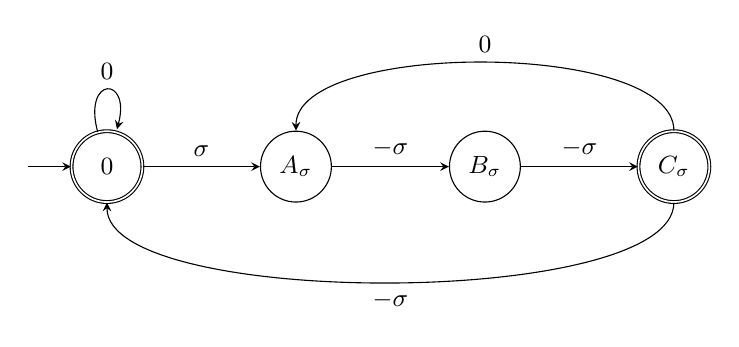
\begin{tikzpicture}[>=stealth, every node/.style={font=\small}]
  \node[draw,circle,double,minimum size=9mm] (z) at (0,0) {$0$};
  \node[draw,circle,minimum size=9mm] (a) at (2.4,0) {$A_\sigma$};
  \node[draw,circle,minimum size=9mm] (b) at (4.8,0) {$B_\sigma$};
  \node[draw,circle,double,minimum size=9mm] (c) at (7.2,0) {$C_\sigma$};
  \draw[->] (-1,0) -- (z);
  \draw[->] (z) edge[loop above] node {$0$} (z);
  \draw[->] (z) -- node[above] {$\sigma$} (a);
  \draw[->] (a) -- node[above] {$-\sigma$} (b);
  \draw[->] (b) -- node[above] {$-\sigma$} (c);
  \draw[->] (c.north) .. controls +(0,1.15) and +(0,1.15) ..
             node[above] {$0$} (a.north);
  \draw[->] (c.south) .. controls +(0,-1.35) and +(0,-1.35) ..
             node[below] {$-\sigma$} (z.south);
 \end{tikzpicture}
 \caption{Admissible digits, read from high exponents to low exponents.
 There are two copies of the three nonzero states, one for each sign
 \(\sigma\), sharing state \(0\). Edge labels are digits; double circles
 mark permitted terminal states. A return to \(0\) may be followed by
 either sign.}
 \label{np:automaton}
\end{figure}

Let \(o(d)=\#\{i:d_i\ne0\}\). At a position \(i\) of a block, define
\begin{equation}
 \eta_i=\sum_{\substack{d\text{ admissible}\\d_i\ne0}}
                  \frac{x_*^{o(d)-2}}{o(d)}.
 \label{np:damping}
\end{equation}
The same coefficients are repeated in every block. An admissible nonzero
pattern has at least three nonzero digits, so all summands are well defined.

\begin{lemma}[Cost of admissible patterns]\label{np:damping-bounds}
Set
\begin{equation}
 S_*=\left(1+\frac{2x_*^4}{1-x_*^2}\right)^{18}
       \left(1+\frac{2x_*^3}{1-x_*^2}\right)-1.
 \label{np:pattern-cost}
\end{equation}
Then \(S_*<0.081\), and
\begin{equation}
 \begin{gathered}
 \sum_{\substack{d\text{ admissible}\\o(d)>0}}x_*^{o(d)}\le S_*,
 \qquad \eta_i x_*^2\le S_*/3,\\
 \frac{\overline\eta}{1-S_*/3}<0.101,
 \qquad \overline\eta=\frac1{21}\sum_{i\in B_q}\eta_i.
 \end{gathered}
 \label{np:damping-estimates}
\end{equation}
\end{lemma}

\begin{proof}
A completed excursion from \(0\) to \(0\) has the digit string
\[
 [\sigma,-\sigma,-\sigma,(0,-\sigma,-\sigma)^l,-\sigma],
 \qquad l\ge0.
\]
It has \(4+2l\) nonzero digits and can begin in at most \(18\) positions
of a block. An optional final excursion ending at \(C_\sigma\) has the
same form without the last digit; its sign and length determine its
starting position. Ignoring incompatibilities between these choices
overcounts the admissible patterns and gives \eqref{np:pattern-cost}.
At \(x_*=0.199\), the two fractions in that expression are less than
\(0.00327\) and \(0.01642\). The inequality
\((1+a)^{18}\le(1-18a)^{-1}\), valid for \(0\le18a<1\), proves
\(S_*<0.081\) by rational arithmetic.

Since \(o(d)\ge3\), each \(\eta_i x_*^2\le S_*/3\). Summing
\eqref{np:damping} over positions gives
\(\sum_i\eta_i\le S_*/x_*^2\). Thus
\[
 \frac{\overline\eta}{1-S_*/3}
 \le\frac{0.081}{21(0.199)^2(1-0.081/3)}<0.101.
\]
\end{proof}

For the moment fix \(N\), and abbreviate
\(Z_i=Z_i^{(0,N)}\), \(G_i=G_i^{(N)}\), and \(x_i=|G_i|\). Define
\begin{equation}
 h_i=1-\eta_i x_i^2,\qquad
 F_i=h_i\bigl(1+(1-x_i^2)(Z_iG_i+\overline{Z_iG_i})\bigr),
 \qquad i\in J_N.
 \label{np:factors}
\end{equation}
These factors are bounded above and bounded away from zero uniformly in
\(N,i,x_D\). Indeed, \(h_i\ge1-S_*/3\), and the other factor is at
least \(1-2x_*>0\).

\begin{proposition}[Bounded integral]\label{np:integral}
For every \(N\) and every fixed complex coordinate \(x_\alpha\),
\begin{equation}
 \int_\R\psi(x_\beta)\prod_{i\in J_N}F_i(x_D)\,dx_\beta
 \le\int_\R\psi(x_\beta)\,dx_\beta,
 \qquad
 \psi(v)=\left(\frac{\sin(\pi v/10)}{\pi v/10}\right)^2,
 \label{np:integral-bound}
\end{equation}
where \(\psi(0)=1\).
\end{proposition}

\begin{proof}
We use the Fourier convention \(e^{2\pi\mathrm i\xi x_\beta}\).
The nonnegative integrable function \(\psi\) has Fourier transform
supported in \([-0.1,0.1]\), hence in \([-1,1]\). On suppressing the
common frequency factor \(-1/p'(\beta)\), the frequency of \(Z_i\) is
\(\beta^i\). Every phase appearing in \(G_i\) has frequency of absolute
value at most \(\beta^{i-30}\). For the type-1 term this follows from
\[
 \bigl|\beta^{i-33}(\beta^{-3}-1+\beta)\bigr|\le\beta^{i-30}.
\]
We call these predictor frequencies slow. Expanding a factor \(F_i\)
gives monomials with one fast digit \(d_i\in\{-1,0,1\}\), corresponding
to \(Z_i^{d_i}\), and at most five slow frequencies: two from \(h_i\),
two from \(1-|G_i|^2\), and one from \(G_i\) or its conjugate.

Expand the last block according to its fast digits, keeping all earlier
factors for the moment. We first show that every inadmissible pattern
has zero integral, even after multiplication by those earlier factors.
Expand the latter and all slow pieces into monomials. If the current
index is \(i\), the fast sum accumulated from the top of the last block,
divided by \(\beta^i\), follows the recurrence
\(v\mapsto\beta v+d_i\). By \eqref{np:near-cubic},
each allowed transition agrees with the state values
\eqref{np:state-values} up to an injected error of absolute value at most
\(\beta^{-30}\). The propagated error, including at a first forbidden
step, is bounded by
\begin{equation}
 \frac{\beta^{-30}\beta^{21}}{\beta-1}<0.005.
 \label{np:recurrence-error}
\end{equation}

At a first forbidden step, the ideal absolute value is at least
\(\beta(\beta-1)\) for a departure from \(A_\sigma\) or \(B_\sigma\),
and at least \(2\) for a departure from \(C_\sigma\). After
\eqref{np:recurrence-error}, it is greater than \(1.5\). All lower fast
digits together contribute at most \((\beta-1)^{-1}<1.192\) in the same
units. If instead all transitions are allowed but the terminal state is
\(A_\sigma\) or \(B_\sigma\), the absolute value at the bottom index
\(i\) is at least \(\beta-1-0.005\). The one-index gap then bounds the
earlier fast terms by \(1/(\beta(\beta-1))<0.649\).

In either case, all slow terms, including those from earlier blocks,
contribute at most
\begin{equation}
 \frac{5\beta^{-30}\beta^{21}}{\beta-1}<0.025
 \label{np:slow-error}
\end{equation}
relative to \(\beta^i\). To see this, sum at most five frequencies of
size \(\beta^{j-30}\) over indices \(j\) no larger than the top of the
last block; that top is at most \(i+20\). Thus the full frequency has
absolute value greater than
\(0.1\beta^i/|p'(\beta)|>1\). Its integral against \(\psi\) is zero.

After removing these zero integrals, the last block contributes
\(\prod_{i\in B_q}h_i\) times the sum over admissible fast patterns.
The zero pattern contributes one. A nonzero pattern has absolute value
at most \(\prod_{d_i\ne0}x_i\), since \(0\le1-x_i^2\le1\).
The arithmetic--geometric mean inequality gives
\[
 \prod_{d_i\ne0}x_i
 \le x_*^{o(d)-2}\frac1{o(d)}\sum_{d_i\ne0}x_i^2.
\]
The absolute value of the retained pattern sum is therefore at most
\(1+\sum_{i\in B_q}\eta_i x_i^2\). Writing \(t_i=\eta_i x_i^2\),
we have \(0\le t_i<1\) and
\[
 \prod_{i\in B_q}(1-t_i)\left(1+\sum_{i\in B_q}t_i\right)\le1;
\]
for example, use \(\prod(1-t_i)\le\exp(-\sum t_i)\).
Since \(\psi\) and all earlier factors are nonnegative, removing the
last block can only increase the upper bound for the integral. Repeat
with the preceding blocks to obtain \eqref{np:integral-bound}.
\end{proof}

\subsection{A typical exponential gain}
\label{np:gain-section}

We now evaluate the same factors in the stationary model, replacing
\(Z_i,G_i\) in \eqref{np:factors} by
\(\mathcal Z_i^{(0)},\mathcal G_i\); denote the resulting factors by
\(\mathcal F_i\). The damping coefficients remain periodic with period
\(22\), and are used at the same \(21\) positions per period.

\begin{lemma}[A logarithmic estimate]\label{np:log-inequality}
For \(0\le x\le x_*\) and \(|u|\le2x\),
\begin{equation}
 \log(1+(1-x^2)u)\ge u-\frac{u^2}{2}-C_*x^3,
 \qquad C_*:=\frac2{3\sqrt{1-x_*^2}}.
 \label{np:log-bound}
\end{equation}
\end{lemma}

\begin{proof}
The assertion is immediate for \(x=0\). Otherwise let
\(D_x(u)=u-u^2/2-\log(1+(1-x^2)u)\). Its derivative is
\[
 D_x'(u)=\frac{x^2-x^2u-(1-x^2)u^2}{1+(1-x^2)u}.
\]
For \(u\ge0\), this is at most the positive part of
\(x^2-(1-x^2)u^2\). Integrating that positive part on \([0,\infty)\)
gives \(2x^3/(3\sqrt{1-x^2})\le C_*x^3\).
On \([-2x,0]\), the only possible interior critical point is a minimum,
so the maximum is at an endpoint. We have \(D_x(0)=0\), whereas
\[
 \frac{d}{dx}D_x(-2x)
 =\frac{2x^2(1-2x-4x^2)}{1-2x+2x^3}\le2x^2.
\]
As \(D_0(0)=0\), integration gives
\(D_x(-2x)\le2x^3/3\le C_*x^3\).
\end{proof}

\begin{proposition}[Growth on typical words]\label{np:typical-gain}
For uniformly distributed words \(a\in\{0,1\}^N\),
\begin{equation}
 \Pr\left\{\sum_{i\in J_N}\log F_i(x(a))>0.000220N\right\}
 \longrightarrow1.
 \label{np:typical-gain-bound}
\end{equation}
\end{proposition}

\begin{proof}
Apply Lemma~\ref{np:log-inequality} with
\(x=|\mathcal G_i|\) and \(u=2\mathcal L_i\). The identity
\[
 2\E\mathcal L_i^2
 =\E|\mathcal G_i|^2+
   \operatorname{Re}\E\bigl[(\mathcal Z_i^{(0)})^2\mathcal G_i^2\bigr]
\]
and the bound \(\E|\mathcal G_i|^3\le x_*\E|\mathcal G_i|^2\)
control the second and third order terms. Also
\[
 \log(1-\eta_i|\mathcal G_i|^2)
 \ge-\frac{\eta_i|\mathcal G_i|^2}{1-S_*/3}.
\]
Set \(\gamma=22^{-1}\sum_{i\in B_0}\E\log\mathcal F_i\), where the
division by \(22\) includes the unused index. Since \(C_*x_*<0.136\),
Proposition~\ref{np:moments} and Lemma~\ref{np:damping-bounds} give the
stationary mean rate \(\gamma\) with
\begin{equation}
 \begin{split}
 \gamma
 &\ge\frac{21}{22}\left(
     2\E\mathcal L_0
     -\left(1+C_*x_*+\frac{\overline\eta}{1-S_*/3}\right)
            \E|\mathcal G_0|^2
     -\left|\E[(\mathcal Z_0^{(0)})^2\mathcal G_0^2]\right|
                       \right)\\
 &>\frac{21}{22}\bigl(2(0.000210)-1.237(0.000145)-0.000007\bigr)
   >0.000222.
 \end{split}
 \label{np:mean-gain}
\end{equation}

For completeness, we justify passage from this mean to finite words.
Truncate each sequence \(C_A\) to \([-H,H]\), for a fixed integer \(H\).
The stationary logarithmic block sums formed from these truncated
sequences depend on finitely many bits. They are uniformly bounded,
have the same mean from block to block, and are independent when their
blocks are sufficiently far apart. The variance of an average of
\(Q\) such block sums is therefore \(O_H(Q^{-1})\). Their averages
converge in probability to their means.

Absolute summability of \(C_0,C_1\) makes the truncated characters
uniformly close to the original characters as \(H\to\infty\).
The predictors are finite sums with bounded total absolute weight, and
the factors are uniformly bounded away from zero. Consequently the
logarithms also converge uniformly under this truncation. Letting
\(H\to\infty\) after \(N\to\infty\) proves
\[
 \frac1N\sum_{i\in J_N}\log\mathcal F_i
   \longrightarrow\gamma\qquad\text{in probability}.
\]

Couple the reversed word bits to \((b_0,\ldots,b_{N-1})\) in this
stationary sequence. For fixed \(H\), the truncated finite and
stationary characters used in a factor agree whenever
\(H+2000\le i\le N-1-H\). Only a number of boundary indices depending
on \(H\), not on \(N\), remain. The same uniform approximation thus
shows
\[
 \frac1N\left(
   \sum_{i\in J_N}\log F_i(x(a))
       -\sum_{i\in J_N}\log\mathcal F_i\right)\longrightarrow0
\]
uniformly over the coupled bit sequences. Together with
\eqref{np:mean-gain}, this proves \eqref{np:typical-gain-bound}.
\end{proof}

\subsection{Counting typical vectors and proving singularity}
\label{np:cover-section}

The integral bound applies to continuous coordinates, whereas
Proposition~\ref{np:typical-gain} concerns lattice points. The remaining
step is to thicken each such point by a fixed radius. Normalization in
the expanding directions makes the resulting change in the whole
logarithmic product bounded independently of the word length.

\begin{lemma}[Thickening word vectors]\label{np:thickening}
There are constants \(\rho>0\) and \(C_{\mathrm{thick}}<\infty\), independent of
\(N\), such that the radius-\(\rho\) balls about distinct lattice points
in Lemma~\ref{np:lattice} are disjoint, and, whenever \(y'\) lies in the
ball about \(y(a)\),
\begin{equation}
 \left|\sum_{i\in J_N}\log F_i(x'_D)
       -\sum_{i\in J_N}\log F_i(x_D(a))\right|\le C_{\mathrm{thick}},
 \qquad x'_r=r^{-N}y'_r\quad(r\in D).
 \label{np:thickening-bound}
\end{equation}
\end{lemma}

\begin{proof}
Choose \(\rho\le1\) smaller than half the minimum distance between
distinct points of the lattice. A coordinate change of size at most
one in \(y\) changes the exponent of \(Z_j^{(0,N)}\) by at most
\[
 2\pi\sum_{r\in D}\frac{|r|^{j-N}}{|p'(r)|}.
\]
Every character occurring in \(F_i\), including those in the type-1
term of the predictor, has index at most \(i\). The logarithm of
\(F_i\) is a uniformly Lipschitz function of these unit phases, since
the coefficient sums and damping coefficients are bounded and \(F_i\)
is uniformly positive. Its variation is therefore at most a fixed
constant times \(\sum_{r\in D}|r|^{i-N}\). Finally,
\[
 \sum_{i\in J_N}|r|^{i-N}
 \le\sum_{i=0}^{N-1}|r|^{i-N}
 <\frac1{|r|-1}\qquad(r\in D).
\]
This proves a bound independent of \(N\).
\end{proof}

\begin{proof}[Proof of Theorem~\ref{np:main}]
The root assertion and the fact that \(\beta\) is not Pisot were proved
above. Call a word typical if it satisfies the inequality in
\eqref{np:typical-gain-bound}, and let \(\mathcal Y_N\) be the set of
distinct vectors \(y(a)\) obtained from typical words. Typical words
have probability tending to one. Lemma~\ref{np:thickening} implies that,
for all sufficiently large \(N\), the product \(\prod_{i\in J_N}F_i\)
is at least \(\exp(0.000216N)\) throughout each of the disjoint balls
about \(\mathcal Y_N\).

All these balls lie in fixed bounded boxes in \((x_D,y_I)\)
coordinates, enlarged from those of Lemma~\ref{np:lattice}. In the
real expanding coordinate one may take \(|x_\beta|\le3\).
The function \(\psi\) has a positive minimum on \([-3,3]\).
Integrating first in \(x_\beta\), Proposition~\ref{np:integral} bounds
the integral of the product over this fixed box by a constant
independent of \(N\). The product does not depend on \(y_I\).
Changing back to \(y\) coordinates contributes the Jacobian
\(\mathcal M^N\). Comparing with the disjoint balls, each of the same
positive volume, gives
\begin{equation}
 \#\mathcal Y_N\le C_{\mathrm{count}}
       \exp\bigl((\log\mathcal M-0.000216)N\bigr)
 \label{np:count}
\end{equation}
for a constant \(C_{\mathrm{count}}\).

Let \(\mu\) be the law of \(\sum_{k\ge0}b_k\beta^{-k}\) for independent
fair bits. By reversal in \eqref{np:word-coordinates}, its length-\(N\)
prefix has the distribution of \(\beta x_\beta(a)\). Projecting
\(\mathcal Y_N\) to this coordinate cannot increase its cardinality.
For each resulting prefix value, attach an interval of length
\(\beta^{-N}/(1-\beta^{-1})\), which contains all possible remaining
tails. Their union \(K_N\) is compact, \(\mu(K_N)\to1\), and
\eqref{np:mahler} and \eqref{np:count} give
\begin{equation}
 |K_N|\le C_{\mathrm{cover}}\exp\bigl((0.0002094-0.000216)N\bigr)
       =C_{\mathrm{cover}}e^{-0.0000066N}.
 \label{np:cover-bound}
\end{equation}
Choose a subsequence \(N_j\) with \(\mu(K_{N_j})>1-2^{-j}\).
Then \(\liminf_jK_{N_j}\) has full \(\mu\)-measure and zero Lebesgue
measure. Thus \(\mu\) is singular. Finally,
\[
 \sum_{k\ge0}(2b_k-1)\beta^{-k}
 =2\sum_{k\ge0}b_k\beta^{-k}-\frac1{1-\beta^{-1}},
\]
so its law \(\nu_{1/\beta}\) is an affine image of \(\mu\) and is
singular as well.
\end{proof}

\appendix
\section{A rational certificate for the degree-31 example}
\label{cert:section}

This appendix proves the root bounds in Proposition~\ref{np:roots} and
the predictor estimates in Proposition~\ref{np:moments}.  The root
calculation uses exact rational arithmetic.  The moment calculation
combines finite rational products with an analytic estimate for their
infinite tails.  We specify the rounding and the order of operations so
that the rational weights in~\eqref{cert:weights} are completely determined.
The accompanying script \texttt{verification/verify\_degree31.py} implements
these instructions using only Python integers and rational fractions;
the recurrences below give the complete certificate independently of
that implementation.  Every terminating decimal in this appendix
denotes its exact rational value.

\subsection{Locating all the roots}
\label{cert:roots}\label{cert:root-proof}

Recall the polynomial
\[
 p(t)=\sum_{j=0}^{9}(-t^{3j}+t^{3j+1})-2t^{30}+t^{31}.
\]
Put $E=10^{40}$.  The entries in Table~\ref{cert:root-table} are the real
and imaginary numerators of centers $z=(a+\mathrm i b)/E$.
Include the conjugate of each nonreal center.  Thus the table specifies
$31$ disks, all of radius $\delta=10^{-35}$.
Denote its first and sixth centers by $z_\beta$ and $z_\alpha$,
respectively.

\begin{table}[htbp]
\centering
\begingroup\scriptsize\ttfamily
\begin{tabular}{rr}
\normalfont Real numerator & \normalfont Imaginary numerator\\\hline
18392867573155250211326543340571993487329 & 0\\
-9741384652837567528189111907762645564212 & 960611633124778624015947511546714789832\\
-9390979934023233037686839914141181659013 & 2848063934279278841200845525848576791934\\
-8707010393241200595697704637503228167256 & 4634358961359777463662031763152574795910\\
-7723118558199735333585947045021501410451 & 6250214494152701297733561366714273855663\\
-6480873022754265587670654805348739312397 & 7617033927823246411701558316834470378693\\
-3296776282962928450195355562079974291919 & 9362810613239308448752821856735617305389\\
-1442513481645415489053007250852371013818 & 9733039088635544125591234293715446465839\\
473579005983151143865690217073943282984 & 9759329295153416086962240697595385836176\\
2372858204750359429049351486827380431084 & 9430908396110323024329804770889268443510\\
4184061662454447896993374181551299054853 & 8750376307352230997951514116951420713869\\
5840543823426662247726359012202878127980 & 7733999914049269380846159864123679516166\\
7280042164772721585016920411987150804420 & 6409668313572020921539025901166241650504\\
8444162922855313595050499086097221186662 & 4814843758334683329011653039104490553475\\
9275649862302447872891854755866108397375 & 2996533501299661135726051235425500195711\\
9715324892541617145821300300817663390044 & 1019107767839771580294306582422817927060
\end{tabular}
\endgroup
\caption{Rational centers for the roots; both columns have denominator $10^{40}$.}
\label{cert:root-table}
\end{table}

For a complex number write $\|z\|_1=|\Re z|+|\Im z|$ and
$\|z\|_\infty=\max(|\Re z|,|\Im z|)$.  Exact Horner evaluation gives,
at every displayed center,
\begin{equation}\label{cert:residual}
 |z|<2,\qquad \|p'(z)\|_\infty>1,\qquad
 2\cdot10^{35}\|p(z)\|_1<\|p'(z)\|_\infty.
\end{equation}
Here is an integer prescription for these comparisons.  For
$q(t)=\sum_{j=0}^d q_jt^j$ and the Gaussian integer $Z=Ez$, initialize
$(V,h)=(q_d,1)$ and, for $j=d-1,d-2,\ldots,0$, replace
\[
 h\leftarrow Eh,\qquad V\leftarrow ZV+hq_j.
\]
The final value is $q(z)=V/h$.  Apply this to $p$ and $p'$, and clear
the positive denominators in~\eqref{cert:residual}.  Comparisons of
squared distances give $|z-z'|>.01$ for distinct centers, including
conjugates.  Comparisons of coordinates and squared moduli also give
\begin{equation}\label{cert:center-bounds}
 \begin{gathered}
 1.83928<z_\beta<1.83929,\qquad
 1.0002090<|z_\alpha|^2<1.0002093,\\
 |z|<.9939\quad\hbox{at all other displayed centers}.
 \end{gathered}
\end{equation}
For $|h|=\delta$, the terms of degree at least two in
$p(z+h)-p(z)-p'(z)h$ have total modulus at most
\[
 \delta^2\sum_{j=0}^{31}|p_j|3^j<10^{17}\delta^2.
\]
Indeed, $|z|<2$ and $\delta<1$, so the binomial expansion gives this
bound term by term.  By~\eqref{cert:residual}, the constant term is
less than $|p'(z)|\delta/2$, whereas the displayed remainder is less
than $|p'(z)|\delta/2$.  Rouch\'e's theorem therefore puts exactly one
root, counted with multiplicity, in each disk.  The disks are disjoint
and their number is the degree, so these are all the roots and all are
simple.  The root in the real-centered disk is real by conjugation.
Every other disk misses the real axis, so the remaining roots form
fifteen nonreal conjugate pairs.
The radius $10^{-35}$ and~\eqref{cert:center-bounds} imply every bound
in Proposition~\ref{np:roots}, including $|1/\alpha|<.9999$.

\subsection{Rounded coefficient arrays and finite products}
\label{cert:algorithm}

The numerical inputs are the sequences $C_0,C_1$ defined in the
main text in~\eqref{np:coefficients}.  We approximate their single and paired moments
\begin{equation}\label{cert:exact-moments}
 P_A=\prod_{m\in\mathbb Z}\cos(\pi C_A(m)),\qquad
 P_{AB}^{\sigma}(k)=
 \prod_{m\in\mathbb Z}\cos\bigl(\pi(C_A(m)+\sigma C_B(m+k))\bigr),
\end{equation}
where $A,B\in\{0,1\}$, $\sigma\in\{1,-1\}$, and $k\ge0$.
Both products converge by exponential decay of the coefficients.
The sign notation $+$ and $-$ means $\sigma=1$ and $\sigma=-1$.

We now specify the approximations used to define the weights.  Use
\[
 S=10^{30},\qquad R=3000,\qquad H=100,\qquad K=2000,
 \qquad W=10^9.
\]
For a real rational $x$ set
\[
 [x]=\frac{\lfloor Sx+1/2\rfloor}{S},
\]
and round complex numbers componentwise.  Thus, if $x=u/v$ with
integers $u,v$ and $v>0$, its rounded numerator is
$\lfloor(2Su+v)/(2v)\rfloor$.  Additions, subtractions, conjugation,
and multiplication by an integer are exact unless brackets are
explicitly displayed.  Set
\[
 \pi'=\frac{3141592653589793238462643383279}{S}.
\]
The inequality $|\pi'-\pi|<1/S$ follows by using $30$ terms of the
alternating series for $\arctan(1/5)$ and $10$ for $\arctan(1/239)$
in Machin's identity
$\pi=16\arctan(1/5)-4\arctan(1/239)$.  The total remainder bound is
\[
 \frac{16}{61\cdot5^{61}}+\frac4{21\cdot239^{21}}.
\]
In particular this verification, too, uses rational arithmetic only.

The contracting and expanding roots are denoted by $I$ and $D$, as in
the main text.  For each representative center $z$ first form
$r_z=[1/p'(z)]$, with $p'(z)$ evaluated exactly.  Store a base and a
coefficient as follows:
\begin{equation}\label{cert:base-pairs}
 (a_z,v_z)=
 \begin{cases}
 ([z],r_z),&|z|<1,\\
 ([1/z],-[[1/z]r_z]),&|z|>1.
 \end{cases}
\end{equation}
For a contracting representative, start $v=v_z$ and add $2\Re v$
to $c_0(-1)$, then to $c_0(-2),c_0(-3),\ldots$, replacing
$v\leftarrow[va_z]$ after each addition.  For an expanding
representative do the same on $c_0(0),c_0(1),\ldots$; the multiplier
is $1$ for the real root and $2$ for the nonreal representative.
All arrays start at zero.  Compute $c_0(m)$ on
\[
 -R-K-5\le m\le H+K+5
\]
and define, wherever these three entries are present,
\begin{equation}\label{cert:shift-array}
 c_1(m)=c_0(m+3)-c_0(m)+c_0(m-1).
\end{equation}
These extra endpoint entries ensure that every subsequent use of
$c_1$ lies in its defined range.  The arrays approximate the sequences
$C_0,C_1$ in the main text.

For a rational input $c$ let $g(c),h(c)$ be the following rounded
cosine and sine values.  The displayed loop fixes the order of the
summation.
\begin{verbatim}
x = [pi' c];  y = [x*x]
t = 1;  u = x;  g = t;  h = u
for j = 1,...,50:
    t = [-t*y/(2*j*(2*j-1))]
    u = [-u*y/(2*j*(2*j+1))]
    g = g+t;  h = h+u
return (g,h)
\end{verbatim}
Write $g_A(m)=g(c_A(m))$ and $h_A(m)=h(c_A(m))$.

The only expanding root close to the unit circle is $\alpha$ and its
conjugate.  To treat their long tail, set
\begin{equation}\label{cert:weak-coefficients}
 a=1/\alpha,\qquad u_0=-a/p'(\alpha),\qquad
 u_1=u_0(a^3-1+1/a).
\end{equation}
Their contribution to $C_A(m)$ for $m\ge H$ is
$u_Aa^m+\overline{u_Aa^m}$.  Let $(a',u'_0)$ be the pair in
\eqref{cert:base-pairs} belonging to $z_\alpha$.  Compute
\[
 a'_0=1,\qquad a'_{n+1}=[a'a'_n]\quad(0\le n<K),\qquad
 u'_1=[u'_0(a'_3-1+[1/a'])].
\]
The subscript in $a'_n$ is a power-array index.

For a single moment use $w=u'_A$ and $k=0$.  For a paired moment
of types $A,B\in\{0,1\}$, sign $\sigma\in\{1,-1\}$, and lag
$0\le k\le K$, use
$w=u'_A+\sigma[u'_Ba'_k]$.  In either case the following calculation
returns an approximate moment.  It retains the finite factors
$-R-k\le m<H$, omits the rapidly convergent negative tail, and treats
the positive tail by summing the degree-$2$, $4$, and $6$ terms of
$-\log\cos$ through geometric series.  Their sum is the variable
\texttt{pen}; the divisors $2,12,45$ are the corresponding Taylor
denominators.  To compute $e^{-\texttt{pen}}$, the algorithm first
approximates $e^{-\texttt{pen}/32}$ and then squares five times.
This tail value is computed first, and the finite factors are then
multiplied in increasing order of $m$.  Section~\ref{cert:error}
bounds all omissions and rounding errors.
\begin{verbatim}
U = [w*a'_H]
q_0 = 1;  q_i = [q_{i-1}*U]       for i = 1,...,6
b_0 = 1;  b_i = [b_{i-1}*pi']     for i = 1,...,6
pen = 0
for d = 2,4,6:
    mom = 0
    for j = 0,...,d:
        num = [q_j*conj(q_{d-j})]
        den = 1-[a'_j*conj(a'_{d-j})]
        mom = mom+binomial(d,j)*Re([num/den])
    pen = pen+[b_d*mom/f_d]       (f_2,f_4,f_6) = (2,12,45)
x = [-pen/32];  t = 1;  value = t
for j = 1,...,40:
    t = [t*x/j];  value = value+t
repeat five times: value = [value*value]
for m = -R-k,...,H-1, in increasing order:
    v = g_A(m)                               (single)
    v = [g_A(m)*g_B(m+k)-sigma*h_A(m)*h_B(m+k)] (pair)
    value = [value*v]
return value
\end{verbatim}
Denote the outputs by $\widetilde P_A$ and
$\widetilde P_{AB}^{\sigma}(k)$, respectively.

We use only lags $30\le k\le2000$.  With $s=0$ for $\sigma=1$ and $s=1$ for
$\sigma=-1$, put $r=\widetilde P_{00}^{\sigma}(k)$ and set
\begin{equation}\label{cert:weights}
 w_{ks}=\frac{\operatorname{sgn}(r)}{W}
 \left\lfloor .68W\max(0,|r|-.00026)+\frac12\right\rfloor,
 \qquad 30\le k\le2000.
\end{equation}
Take $\operatorname{sgn}(0)=0$ and omit zero weights from subsequent
sums.  The recurrences above and this formula define the weights
without any choices or numerical tolerances.

\subsection{A uniform error bound for the moment calculation}
\label{cert:error}

We prove
\begin{equation}\label{cert:delta}
 |\widetilde P_A-P_A|<\Delta,
 \qquad
 |\widetilde P_{AB}^{\sigma}(k)-P_{AB}^{\sigma}(k)|<\Delta,
 \qquad \Delta=5\cdot10^{-6},
\end{equation}
for all types, signs, and lags used above.  The important issue is the
weakly contracting base $a=1/\alpha$: truncating its powers at $H=100$
would not be accurate.  The geometric sums in the tail calculation
retain all of these powers.

\paragraph{Coefficient and trigonometric errors.}
For $|z|<2.001$, termwise differentiation gives
\[
 |p''(z)|<4\cdot10^{13}.
\]
Hence $p'$ changes by less than $4\cdot10^{-22}$ between a center
and its root.  By~\eqref{cert:residual}, reciprocal differentiation
and rounding in~\eqref{cert:base-pairs} give base errors less than
$2/S$ and coefficient errors less than $10^{-21}$.  Direct squared
modulus comparisons give $|a_z|<1$ and $|v_z|\le1$ for every stored
pair.  The corresponding exact coefficients have modulus less than
$1.001$.  Thus each recurrence step $v\leftarrow[va_z]$ propagates
the existing error with factor at most $1$ and adds less than $4/S$.
There are fewer than $5100$ such steps in any needed entry.  Each
coefficient-times-power term consequently has error less than
$2\cdot10^{-21}$, and
\begin{equation}\label{cert:coefficient-errors}
 |c_0(m)-C_0(m)|<7\cdot10^{-20},\qquad
 |c_1(m)-C_1(m)|<2.1\cdot10^{-19}.
\end{equation}

The finite recurrence also gives the following rational comparisons:
\begin{equation}\label{cert:array-bounds}
 \begin{gathered}
 \max_{A,m}|c_A(m)|<.847,\qquad
 \max_{m\ge-20}|c_0(m)|<.018,\qquad
 \max_A|u'_A|<.0087,\\
 .8460<\max_{A,m}|c_A(m)|<.8462.
 \end{gathered}
\end{equation}
The maxima here range over the computed entries; use squared
moduli for the complex coefficients $u'_A$.  To reproduce them, perform
the coefficient recurrences in~\eqref{cert:base-pairs}, the additions
in~\eqref{cert:shift-array}, and the displayed definition of $u'_1$.
These comparisons require neither evaluation of trigonometric
functions nor a root-finding routine.

Every later trigonometric input is a sum of at most four of these
coefficients, counted with multiplicity.  Its error is less than
$10^{-18}$, and its rounded angle satisfies $|x|\le13$ and $|y|\le170$.
The angle error is less than $4\cdot10^{-18}$.  For the Taylor
recurrences at a fixed value of $y$, each term-rounding error
contributes at most $e^{14}/S$ to the final sum: the subsequent
factorial denominators bound the amplification by
$\sum_{j\ge0}170^j/(2j)!<e^{14}$.  Replacing $x^2$ by $y$ costs
at most $100e^{14}/S$, by differentiating the absolute term sums.
The omitted Taylor tails at $|x|\le13$ are less than $10^{-30}$.
Together these effects give errors below $10^{-20}$ relative to
the computed angle, and below $10^{-16}$ relative to the true
cosine and sine.  In particular every single or paired finite
factor has error less than $10^{-15}$.

There are at most $R+K+H=5100$ finite factors.  The true factors have
modulus at most $1$, and their approximations have modulus at most
$1+10^{-15}$.  Telescoping the product, including its roundings,
shows that with an initial value of modulus at most $2$ these errors
contribute less than $3\cdot10^{-11}$.

\paragraph{Terms omitted at the two ends.}
On the negative side, $|C_0(m)|\le32(.994)^{-1-m}$ for $m<0$,
by summing the contracting-root terms.  Including the three shifts
for type $1$, a single or paired coefficient at $m<-R-k$ is bounded by
\[
 200(.994)^{-4-(m+k)}.
\]
Using $1-\cos u\le u^2/2$ and telescoping products, the total omitted
product costs at most
\[
 \frac{3.142^2\,200^2}{2}
 \frac{(.994)^{5994}}{1-(.994)^2}<5\cdot10^{-8}.
\]
For example, the rational inequality $(.994)^{2996}<3\cdot10^{-8}$
already suffices for this estimate.  On the positive side the only
terms omitted from the coefficients are those from $\beta$.
Their bases are less than $.545$, and their type-$0$ and type-$1$
coefficients have modulus at most $4$.  The cosine Lipschitz bound
therefore gives a total error at most
$3.142\cdot8\cdot(.545)^{100}/(1-.545)<10^{-20}$.

\paragraph{The geometric tail and its rounding.}
Let $w_*=u_A$ in the single case and
$w_*=u_A+\sigma u_Ba^k$ in the paired case.  Put $U_*=w_*a^H$.
The exact sums of the even powers of the weak-root tail are
\begin{equation}\label{cert:geometric-moments}
 \mu_d=\sum_{n\ge0}(U_*a^n+\overline{U_*a^n})^d
 =\sum_{j=0}^d\binom dj\Re
 \frac{U_*^j\overline{U_*}^{d-j}}{1-a^j\bar a^{d-j}}
 \quad(d=2,4,6).
\end{equation}
The equality follows by the binomial theorem and absolutely
convergent geometric series.  In particular $\mu_d\ge0$.

The power-array errors satisfy $|a'_n-a^n|\le3n/S$.  Because
$|a|,|a'|>.99$, the formula for $u'_1$ gives errors below
$5\cdot10^{-21}$ for both $u'_A$, and $|u_A|\le.00871$.
It follows that the computed $U$ has error below $10^{-19}$;
its powers through degree $6$ have errors below $10^{-18}$.
In each quotient in the algorithm, the numerator error is below
$3\cdot10^{-18}$ and the denominator error is below $10^{-28}$.
The true and computed denominators have modulus greater than
$.00019$: use
\[
 |1-a^j\bar a^{d-j}|\ge1-|a|^d
 >1-(.9999)^2>.00019
\]
and the stated rounding error.  Hence each quotient error is below
$2\cdot10^{-14}$, the error in each computed $\mu_d$ is below
$2\cdot10^{-12}$, and $|\mu_d|<4\cdot10^5$ by the same denominator
bound.  The rounded powers of $\pi'$ through degree $6$ have errors
below $10^{-22}$.  Consequently \texttt{pen} approximates the
nonnegative number
\begin{equation}\label{cert:penalty}
 P=\frac{\pi^2\mu_2}{2}+\frac{\pi^4\mu_4}{12}
       +\frac{\pi^6\mu_6}{45}
\end{equation}
to within $10^{-9}$.

For $m\ge H$, the weak coefficient has angle bounded by
\[
 3.142\cdot4\cdot.00871\cdot(.9999)^m
 <.11(.9999)^m.
\]
Summing the powers of this bound gives
\[
 P\le\frac{.11^2}{2(1-.9999^2)}
      +\frac{.11^4}{12(1-.9999^4)}
      +\frac{.11^6}{45(1-.9999^6)}<31.
\]
Thus $|\texttt{pen}|<32$ and $|x|<1.1$ in the exponential
calculation.  The $40$-term exponential recurrence has Taylor
remainder less than $10^{-40}$.  Its rounding errors, bounded using
$e^{1.1}$, are negligible compared with $10^{-9}$.  Each squaring
amplifies its existing error by at most $3$, since the true
intermediate values for the computed penalty are at most
$e^{10^{-9}}$.  Including the error in~\eqref{cert:penalty}, the
returned exponential is within $4\cdot10^{-9}$ of $e^{-P}$.

\paragraph{The analytic remainder of the tail.}
For real $z$ with $|z|\le.11$ one has
\begin{equation}\label{cert:logcos-remainder}
 \left| -\log\cos z-\frac{z^2}{2}-\frac{z^4}{12}
                         -\frac{z^6}{45}\right|\le.1z^8.
\end{equation}
Here are elementary bounds proving the stated constant.  Set
$y=z^2$, $h=1-\cos z$, and
$h_0=y/2-y^2/24+y^3/720$.  Then $0\le h\le y/2$ and
$|h-h_0|\le y^4/40320$.  In
$-\log(1-h)=h+h^2/2+h^3/3+\cdots$, the terms after the third
are bounded by $h^4/(4(1-h))<.016y^4$.  Substitution of $h_0$
in the first three terms costs less than $.00004y^4$.
The terms through degree $3$ are $y/2+y^2/12+y^3/45$;
the sum of the absolute values of the remaining coefficients is
less than $.03$, so their contribution is less than $.03y^4$
for $0\le y\le.0121$.  These bounds imply~\eqref{cert:logcos-remainder}.

Applying~\eqref{cert:logcos-remainder} to all weak tail angles gives
\[
 \left|\sum_{m\ge H}-\log\cos
       \bigl(\pi(w_*a^m+\overline{w_*a^m})\bigr)-P\right|
 \le\frac{.1(.11)^8}{1-(.9999)^8}<3\cdot10^{-6}.
\]
Both penalties are nonnegative, so the same bound applies to the
difference of their exponentials.  Combining this with the rounding
error, the finite-factor error, and the two omitted ends proves
\eqref{cert:delta}; indeed the sum of the stated errors is below
$3.055\cdot10^{-6}$.

\subsection{Correlation, variance, and the absolute Gram sum}
\label{cert:moments}\label{cert:moment-proof}

For the rest of the appendix, abbreviate
$Z_i=\mathcal Z_i^{(0)}$ and $G_i=\mathcal G_i$ from
\eqref{np:stationary} and~\eqref{np:predictor}.  All expectations are
under the stationary law of the two-sided independent bits.

The preceding calculation defines exact rational weights and bounds
each moment error uniformly.  We next sum those moments to prove
the first three estimates of Proposition~\ref{np:moments}.  A final
finite-product estimate will prove the fourth.

Write $X=-.001$, $Y=.0055$, and let $\mathcal R$ be the nonzero
rows $(w_{ks},k,s)$ with $30\le k\le2000$.  Define
\[
 b_A=\widetilde P_A,\qquad
 m_{k0}=\widetilde P_{00}^{+}(k),\quad
 m_{k1}=\widetilde P_{00}^{-}(k),\qquad
 e=\widetilde P_{01}^{+}(33).
\]
The approximated correlation is
\begin{equation}\label{cert:corr-sum}
 \widetilde c=Xb_0+Ye+\sum_{(w,k,s)\in\mathcal R}wm_{ks}.
\end{equation}
For each lag $k$, let $J_{k0}$ and $J_{k1}$ be respectively the
second (minus) and first (plus) entries of the following pair:
\[
 \begin{cases}
 (\widetilde P_{10}^{+}(k-33),\widetilde P_{10}^{-}(k-33)),&k\ge33,\\
 (\widetilde P_{01}^{+}(33-k),\widetilde P_{01}^{-}(33-k)),&k<33.
 \end{cases}
\]
The approximated squared norm and absolute Gram sum are
\begin{align}
 \widetilde v={}&X^2+Y^2+2XYb_1
 +2\sum_{(w,k,s)\in\mathcal R}w(Xb_0+YJ_{ks})
 \notag\\[-2pt]
 &+\sum_{(w,k,s),(v,l,t)\in\mathcal R}
           wv\,m_{|k-l|,\,\mathbf1_{s=t}},\label{cert:var-sum}\\
 \widetilde T={}&
 \sum_{\substack{(w,k,s),(v,l,t)\in\mathcal R\\k,l\ge50}}
       |wv\,m_{|k-l|,\,\mathbf1_{s=t}}|.\label{cert:T-sum}
\end{align}
Both double sums are over ordered pairs.  Equal signs require the
minus moment in a conjugated phase pair; opposite signs require the
plus moment.  This explains the index $\mathbf1_{s=t}$, including
the diagonal cases.

The exact finite calculations give
\begin{equation}\label{cert:exact-output}
 \begin{aligned}
 |\mathcal R|&=753,\\
 |X|+|Y|+\sum_{\mathcal R}|w|&=198442946/W,\\
 |X|+|Y|+\sum_{\substack{(w,k,s)\in\mathcal R\\k<50}}|w|
     &=11816095/W,\\
 WS\widetilde c&=211815537786494774284357596751188225,\\
 W^2S\widetilde v&=143920884250294630908494564120361905955993456,\\
 W^2S\widetilde T&=105303788239450118397416374596041413014338334.
 \end{aligned}
\end{equation}
These are integer equalities: compute the arrays and products in
Section~\ref{cert:algorithm}, round the weights by~\eqref{cert:weights},
and use the unrounded rational sums
\eqref{cert:corr-sum}--\eqref{cert:T-sum}.  In particular
\[
 211810<10^9\widetilde c<211820,\quad
 143910<10^9\widetilde v<143930,\quad
 105300<10^9\widetilde T<105310.
\]
This gives $|G_i|<.199$ and $|G_i^{(N)}(x)|<.199$ by the triangle
inequality.  The total
correlation error is at most $\Delta\cdot.199$, and the squared-norm
error is at most $\Delta\cdot.199^2$.  Thus
\[
 \mathbb E\Re(Z_iG_i)>.0002108205>.000210,
 \qquad
 \mathbb E|G_i|^2<.000144119<.000145.
\]

To prepare for the last estimate, call the constant row, the type-$1$
row, and the rows with $k<50$ the \emph{small rows}; the remaining
rows are the \emph{big rows}.  A row of weight $w_v$ has phase
$U_v=\exp(\pi\mathrm i\sum_m f_v(m)e_m)$, where
$e_m=2b_{i+m}-1$.  Its sequence $f_v$ is zero for the constant,
$C_1(m+33)$ for the type-$1$ row, and
$(1-2s)C_0(m+k)$ for a row $(w,k,s)$.  Define the true absolute
Gram sum
\begin{equation}\label{cert:true-T}
 T=\sum_{v,v'\ {\rm big}}|w_vw_{v'}\mathbb E U_v\overline{U_{v'}}|.
\end{equation}
The error between this sum and~\eqref{cert:T-sum} is at most
$\Delta\cdot.199^2$, by $||x|-|y||\le|x-y|$.  Hence
\begin{equation}\label{cert:T-bound}
 T<.000116,\qquad \sqrt T<.011.
\end{equation}
The total absolute weight of the small rows is less than $.012$.

\subsection{Finite products controlling the remaining moment}
\label{cert:finite-products}

We now bound $\mathbb E(Z_i^2G_i^2)$.  The big rows have small
coefficients on the $71$ positions $-70\le m\le0$.  More precisely,
with $t=.06$, \eqref{cert:coefficient-errors} and
\eqref{cert:array-bounds} give
\begin{equation}\label{cert:tangent-bound}
 |\tan(\pi f_v(m))|\le t
 \quad(v\hbox{ big},\ -70\le m\le0).
\end{equation}
Indeed $m+k\ge-20$ for these rows, and the coefficient bound $.018$,
together with $\sin u\le u$ and $\cos u\ge1-u^2/2$, is sufficient.

For any real sequence $V$ put $c_m=|\cos(\pi V(m))|$ and
$s_m=|\sin(\pi V(m))|$.  The finite products needed below are
\begin{align}
 B_2(V)&=\prod_{m=-70}^0
  \min\left(1,\frac{(1+t^2)c_m+2ts_m}{1-t^2}\right),\notag\\
 B_1(V)&=\prod_{m=-70}^0
  \min\left(1,\frac{c_m+ts_m}{\sqrt{1-t^2}}\right),\label{cert:B-def}\\
 B_0(V)&=\prod_{m=-200}^0c_m.\notag
\end{align}
Their bounds are
\begin{equation}\label{cert:B-bounds}
 B_2(2C_0)<.011,\qquad
 \max_{f\ {\rm small}}B_1(2C_0+f)<.015,\qquad
 \max_{f,g\ {\rm small}}B_0(2C_0+f+g)<.0032.
\end{equation}
Here the maxima range over the actual phase sequences of the small
rows.  Besides the constant and the type-$1$ row, their eight
nonzero rows are as follows:
\[
\begin{array}{c|rrrrrrrr}
 k&32&36&37&39&40&43&44&47\\
 s&0&1&0&1&0&0&1&1\\
 Ww_{ks}&-536932&1265024&331701&47119&1483338&436861&458216&756904
\end{array}
\]

For completeness, the following upper-rounding calculation verifies
all of~\eqref{cert:B-bounds}.  For each of its three cases and each
indicated choice of small rows, form the approximate sequence $V'$
by replacing $C_A$ by $c_A$.  Initialize $v=1$.  For increasing $m$
in the relevant interval, compute
\begin{align*}
 b&=|g(V'(m))|+10^{-15},& y&=|h(V'(m))|+10^{-15},\\
 F_0&=b,&
 F_1&=S^{-1}+[1.002(b+.06y)],\\
 &&F_2&=S^{-1}+[1.004(1.0036b+.12y)],\\
 v&\leftarrow S^{-1}+[v\min(1,F_j)]&&\text{in case }j.
\end{align*}
The factors $1.002$ and $1.004$ bound
$(1-t^2)^{-1/2}$ and $(1-t^2)^{-1}$, respectively.  The added
$10^{-15}$ exceeds the trigonometric error proved above, and each
added $S^{-1}$ compensates for a possibly downward rounding.
Thus this calculation gives upper bounds, including for $B_0$
because its true factors are at most $1$.  The maximum final
numerators at scale $S$, in the order $B_2,B_1,B_0$, are
\begin{equation}\label{cert:B-output}
 \begin{gathered}
 10861284406435197401851134503,\\
 14731866010915969694738277129,\\
 3155364376927094122833206055.
 \end{gathered}
\end{equation}
Multiplication by $10^6/S$ bounds them respectively by $10862$,
$14732$, and $3156$, proving~\eqref{cert:B-bounds}.

\subsection{From the finite products to the anisotropy bound}
\label{cert:walsh}

The estimates just obtained concern individual coefficients and
finite products.  We finish by showing how they control the full
sum of phases without expanding every three-phase moment.
Write $G_i=G_{\rm small}+G_{\rm big}$ according to the preceding
partition, and fix any subset $J\subset\{-70,\ldots,0\}$.
Expanding the big phases in the independent signs $e_m$ on $J$ gives
\begin{equation}\label{cert:walsh-expansion}
 G_{\rm big}=\sum_{A\subset J}\mathrm i^{|A|}e_AH_A,
 \qquad e_A=\prod_{m\in A}e_m,
\end{equation}
where
\[
 H_A=\sum_{v\ {\rm big}}w_vU_v^{\rm out}
       \prod_{m\in J}\cos(\pi f_v(m))
       \prod_{m\in A}\tan(\pi f_v(m)).
\]
The phase $U_v^{\rm out}$ depends only on signs outside $J$, so
each $H_A$ is independent of the signs on $J$.

We claim that
\begin{equation}\label{cert:H-bound}
 \|H_A\|_2\le\sqrt T\,t^{|A|}(1-t^2)^{-|J|/2}.
\end{equation}
For two big rows, independence gives their full Gram entry as the
outside Gram entry times
\[
 \prod_{m\in J}\cos(\pi f_v(m))\cos(\pi f_{v'}(m))
       \bigl(1+\tan(\pi f_v(m))\tan(\pi f_{v'}(m))\bigr).
\]
By~\eqref{cert:tangent-bound}, each last factor is at least $1-t^2$.
In the expansion of $\|H_A\|_2^2$, the extra tangent products have
modulus at most $t^{2|A|}$.  Taking absolute values term by term
therefore bounds the squared norm by
$Tt^{2|A|}(1-t^2)^{-|J|}$, proving~\eqref{cert:H-bound}.

First consider $\mathbb E(Z_i^2G_{\rm big}^2)$ and set $V=2C_0$.
For a pair $A,A'\subset J$ in~\eqref{cert:walsh-expansion},
averaging the signs on $J$ contributes a factor of modulus $c_m$
where membership in $A,A'$ agrees, and a factor of modulus $s_m$
where it differs.  The outside expectation is bounded by
$\|H_A\|_2\|H_{A'}\|_2$ using Cauchy--Schwarz and the unit modulus
of the outside part of $Z_i^2$.  Summing over the four membership
choices at each site gives
\[
 |\mathbb E(Z_i^2G_{\rm big}^2)|
 \le T\prod_{m\in J}\frac{(1+t^2)c_m+2ts_m}{1-t^2}.
\]
Choose $J$ to contain precisely those positions whose displayed
factor is less than $1$.  This yields
\begin{equation}\label{cert:big-square}
 |\mathbb E(Z_i^2G_{\rm big}^2)|\le T B_2(2C_0).
\end{equation}

For a fixed small phase $U$ with sequence $f$, use the same expansion
with $V=2C_0+f$.  There is now one subset $A$; summing its two
membership choices produces $c_m+ts_m$.  The outside expectation
is bounded by $\|H_A\|_2$.  Optimizing $J$ as before gives
\[
 |\mathbb E(Z_i^2UG_{\rm big})|
 \le\sqrt T B_1(2C_0+f).
\]
For two small phases with sequences $f,g$, independence directly
bounds their full moment by $B_0(2C_0+f+g)$: discard all the other
absolute cosine factors, which are at most $1$.

Finally sum these bounds with the absolute row weights.  Using
\eqref{cert:T-bound}, \eqref{cert:B-bounds}, and the small-weight
bound $.012$, we obtain
\[
 \begin{split}
 |\mathbb E(Z_i^2G_i^2)|
 &\le T\cdot.011+2(.012)\sqrt T\cdot.015
                           +(.012)^2\cdot.0032\\
 &<.000116\cdot.011+2\cdot.012\cdot.011\cdot.015
                           +.012^2\cdot.0032\\
 &=.0000056968<.000007.
 \end{split}
\]
This proves the remaining estimate of Proposition~\ref{np:moments}.

\begingroup\small
\bibliographystyle{plainnat}
\bibliography{references}
\endgroup
\end{document}
